
%% bare_adv.tex
%% V1.4b
%% 2015/08/26
%% by Michael Shell
%% See: 
%% http://www.michaelshell.org/
%% for current contact information.
%%
%% This is a skeleton file demonstrating the advanced use of IEEEtran.cls
%% (requires IEEEtran.cls version 1.8b or later) with an IEEE Computer
%% Society journal paper.
%%
%% Support sites:
%% http://www.michaelshell.org/tex/ieeetran/
%% http://www.ctan.org/pkg/ieeetran
%% and
%% http://www.ieee.org/

%%*************************************************************************
%% Legal Notice:
%% This code is offered as-is without any warranty either expressed or
%% implied; without even the implied warranty of MERCHANTABILITY or
%% FITNESS FOR A PARTICULAR PURPOSE! 
%% User assumes all risk.
%% In no event shall the IEEE or any contributor to this code be liable for
%% any damages or losses, including, but not limited to, incidental,
%% consequential, or any other damages, resulting from the use or misuse
%% of any information contained here.
%%
%% All comments are the opinions of their respective authors and are not
%% necessarily endorsed by the IEEE.
%%
%% This work is distributed under the LaTeX Project Public License (LPPL)
%% ( http://www.latex-project.org/ ) version 1.3, and may be freely used,
%% distributed and modified. A copy of the LPPL, version 1.3, is included
%% in the base LaTeX documentation of all distributions of LaTeX released
%% 2003/12/01 or later.
%% Retain all contribution notices and credits.
%% ** Modified files should be clearly indicated as such, including  **
%% ** renaming them and changing author support contact information. **
%%*************************************************************************


% *** Authors should verify (and, if needed, correct) their LaTeX system  ***
% *** with the testflow diagnostic prior to trusting their LaTeX platform ***
% *** with production work. The IEEE's font choices and paper sizes can   ***
% *** trigger bugs that do not appear when using other class files.       ***                          ***
% The testflow support page is at:
% http://www.michaelshell.org/tex/testflow/


% IEEEtran V1.7 and later provides for these CLASSINPUT macros to allow the
% user to reprogram some IEEEtran.cls defaults if needed. These settings
% override the internal defaults of IEEEtran.cls regardless of which class
% options are used. Do not use these unless you have good reason to do so as
% they can result in nonIEEE compliant documents. User beware. ;)
%
%\newcommand{\CLASSINPUTbaselinestretch}{1.0} % baselinestretch
%\newcommand{\CLASSINPUTinnersidemargin}{1in} % inner side margin
%\newcommand{\CLASSINPUToutersidemargin}{1in} % outer side margin
%\newcommand{\CLASSINPUTtoptextmargin}{1in}   % top text margin
%\newcommand{\CLASSINPUTbottomtextmargin}{1in}% bottom text margin




%
\documentclass[10pt,journal,compsoc]{IEEEtran}
% If IEEEtran.cls has not been installed into the LaTeX system files,
% manually specify the path to it like:
% \documentclass[10pt,journal,compsoc]{../sty/IEEEtran}


% For Computer Society journals, IEEEtran defaults to the use of 
% Palatino/Palladio as is done in IEEE Computer Society journals.
% To go back to Times Roman, you can use this code:
%\renewcommand{\rmdefault}{ptm}\selectfont





% Some very useful LaTeX packages include:
% (uncomment the ones you want to load)

%%%%%%%
%\usepackage{biblatex}
%\addbibresource{IEEEexamples}

%%%%%%%



% *** MISC UTILITY PACKAGES ***
%
%\usepackage{ifpdf}
% Heiko Oberdiek's ifpdf.sty is very useful if you need conditional
% compilation based on whether the output is pdf or dvi.
% usage:
% \ifpdf
%   % pdf code
% \else
%   % dvi code
% \fi
% The latest version of ifpdf.sty can be obtained from:
% http://www.ctan.org/pkg/ifpdf
% Also, note that IEEEtran.cls V1.7 and later provides a builtin
% \ifCLASSINFOpdf conditional that works the same way.
% When switching from latex to pdflatex and vice-versa, the compiler may
% have to be run twice to clear warning/error messages.






% *** CITATION PACKAGES ***
%
\ifCLASSOPTIONcompsoc
  % The IEEE Computer Society needs nocompress option
  % requires cite.sty v4.0 or later (November 2003)
  \usepackage[nocompress]{cite}
\else
  % normal IEEE
  \usepackage{cite}
\fi
% cite.sty was written by Donald Arseneau
% V1.6 and later of IEEEtran pre-defines the format of the cite.sty package
% \cite{} output to follow that of the IEEE. Loading the cite package will
% result in citation numbers being automatically sorted and properly
% "compressed/ranged". e.g., [1], [9], [2], [7], [5], [6] without using
% cite.sty will become [1], [2], [5]--[7], [9] using cite.sty. cite.sty's
% \cite will automatically add leading space, if needed. Use cite.sty's
% noadjust option (cite.sty V3.8 and later) if you want to turn this off
% such as if a citation ever needs to be enclosed in parenthesis.
% cite.sty is already installed on most LaTeX systems. Be sure and use
% version 5.0 (2009-03-20) and later if using hyperref.sty.
% The latest version can be obtained at:
% http://www.ctan.org/pkg/cite
% The documentation is contained in the cite.sty file itself.
%
% Note that some packages require special options to format as the Computer
% Society requires. In particular, Computer Society  papers do not use
% compressed citation ranges as is done in typical IEEE papers
% (e.g., [1]-[4]). Instead, they list every citation separately in order
% (e.g., [1], [2], [3], [4]). To get the latter we need to load the cite
% package with the nocompress option which is supported by cite.sty v4.0
% and later.





% *** GRAPHICS RELATED PACKAGES ***
%
\ifCLASSINFOpdf
  % \usepackage[pdftex]{graphicx}
  % declare the path(s) where your graphic files are
  % \graphicspath{{../pdf/}{../jpeg/}}
  % and their extensions so you won't have to specify these with
  % every instance of \includegraphics
  % \DeclareGraphicsExtensions{.pdf,.jpeg,.png}
\else
  % or other class option (dvipsone, dvipdf, if not using dvips). graphicx
  % will default to the driver specified in the system graphics.cfg if no
  % driver is specified.
  % \usepackage[dvips]{graphicx}
  % declare the path(s) where your graphic files are
  % \graphicspath{{../eps/}}
  % and their extensions so you won't have to specify these with
  % every instance of \includegraphics
  % \DeclareGraphicsExtensions{.eps}
\fi
% graphicx was written by David Carlisle and Sebastian Rahtz. It is
% required if you want graphics, photos, etc. graphicx.sty is already
% installed on most LaTeX systems. The latest version and documentation
% can be obtained at: 
% http://www.ctan.org/pkg/graphicx
% Another good source of documentation is "Using Imported Graphics in
% LaTeX2e" by Keith Reckdahl which can be found at:
% http://www.ctan.org/pkg/epslatex
%
% latex, and pdflatex in dvi mode, support graphics in encapsulated
% postscript (.eps) format. pdflatex in pdf mode supports graphics
% in .pdf, .jpeg, .png and .mps (metapost) formats. Users should ensure
% that all non-photo figures use a vector format (.eps, .pdf, .mps) and
% not a bitmapped formats (.jpeg, .png). The IEEE frowns on bitmapped formats
% which can result in "jaggedy"/blurry rendering of lines and letters as
% well as large increases in file sizes.
%
% You can find documentation about the pdfTeX application at:
% http://www.tug.org/applications/pdftex





% *** MATH PACKAGES ***
%
%\usepackage{amsmath}
% A popular package from the American Mathematical Society that provides
% many useful and powerful commands for dealing with mathematics.
%
% Note that the amsmath package sets \interdisplaylinepenalty to 10000
% thus preventing page breaks from occurring within multiline equations. Use:
%\interdisplaylinepenalty=2500
% after loading amsmath to restore such page breaks as IEEEtran.cls normally
% does. amsmath.sty is already installed on most LaTeX systems. The latest
% version and documentation can be obtained at:
% http://www.ctan.org/pkg/amsmath





% *** SPECIALIZED LIST PACKAGES ***
%\usepackage{acronym}
% acronym.sty was written by Tobias Oetiker. This package provides tools for
% managing documents with large numbers of acronyms. (You don't *have* to
% use this package - unless you have a lot of acronyms, you may feel that
% such package management of them is bit of an overkill.)
% Do note that the acronym environment (which lists acronyms) will have a
% problem when used under IEEEtran.cls because acronym.sty relies on the
% description list environment - which IEEEtran.cls has customized for
% producing IEEE style lists. A workaround is to declared the longest
% label width via the IEEEtran.cls \IEEEiedlistdecl global control:
%
% \renewcommand{\IEEEiedlistdecl}{\IEEEsetlabelwidth{SONET}}
% \begin{acronym}
%
% \end{acronym}
% \renewcommand{\IEEEiedlistdecl}{\relax}% remember to reset \IEEEiedlistdecl
%
% instead of using the acronym environment's optional argument.
% The latest version and documentation can be obtained at:
% http://www.ctan.org/pkg/acronym


%\usepackage{algorithmic}
% algorithmic.sty was written by Peter Williams and Rogerio Brito.
% This package provides an algorithmic environment fo describing algorithms.
% You can use the algorithmic environment in-text or within a figure
% environment to provide for a floating algorithm. Do NOT use the algorithm
% floating environment provided by algorithm.sty (by the same authors) or
% algorithm2e.sty (by Christophe Fiorio) as the IEEE does not use dedicated
% algorithm float types and packages that provide these will not provide
% correct IEEE style captions. The latest version and documentation of
% algorithmic.sty can be obtained at:
% http://www.ctan.org/pkg/algorithms
% Also of interest may be the (relatively newer and more customizable)
% algorithmicx.sty package by Szasz Janos:
% http://www.ctan.org/pkg/algorithmicx




% *** ALIGNMENT PACKAGES ***
%
%\usepackage{array}
% Frank Mittelbach's and David Carlisle's array.sty patches and improves
% the standard LaTeX2e array and tabular environments to provide better
% appearance and additional user controls. As the default LaTeX2e table
% generation code is lacking to the point of almost being broken with
% respect to the quality of the end results, all users are strongly
% advised to use an enhanced (at the very least that provided by array.sty)
% set of table tools. array.sty is already installed on most systems. The
% latest version and documentation can be obtained at:
% http://www.ctan.org/pkg/array


%\usepackage{mdwmath}
%\usepackage{mdwtab}
% Also highly recommended is Mark Wooding's extremely powerful MDW tools,
% especially mdwmath.sty and mdwtab.sty which are used to format equations
% and tables, respectively. The MDWtools set is already installed on most
% LaTeX systems. The lastest version and documentation is available at:
% http://www.ctan.org/pkg/mdwtools


% IEEEtran contains the IEEEeqnarray family of commands that can be used to
% generate multiline equations as well as matrices, tables, etc., of high
% quality.


%\usepackage{eqparbox}
% Also of notable interest is Scott Pakin's eqparbox package for creating
% (automatically sized) equal width boxes - aka "natural width parboxes".
% Available at:
% http://www.ctan.org/pkg/eqparbox




% *** SUBFIGURE PACKAGES ***
%\ifCLASSOPTIONcompsoc
%  \usepackage[caption=false,font=footnotesize,labelfont=sf,textfont=sf]{subfig}
%\else
%  \usepackage[caption=false,font=footnotesize]{subfig}
%\fi
% subfig.sty, written by Steven Douglas Cochran, is the modern replacement
% for subfigure.sty, the latter of which is no longer maintained and is
% incompatible with some LaTeX packages including fixltx2e. However,
% subfig.sty requires and automatically loads Axel Sommerfeldt's caption.sty
% which will override IEEEtran.cls' handling of captions and this will result
% in non-IEEE style figure/table captions. To prevent this problem, be sure
% and invoke subfig.sty's "caption=false" package option (available since
% subfig.sty version 1.3, 2005/06/28) as this is will preserve IEEEtran.cls
% handling of captions.
% Note that the Computer Society format requires a sans serif font rather
% than the serif font used in traditional IEEE formatting and thus the need
% to invoke different subfig.sty package options depending on whether
% compsoc mode has been enabled.
%
% The latest version and documentation of subfig.sty can be obtained at:
% http://www.ctan.org/pkg/subfig




% *** FLOAT PACKAGES ***
%
%\usepackage{fixltx2e}
% fixltx2e, the successor to the earlier fix2col.sty, was written by
% Frank Mittelbach and David Carlisle. This package corrects a few problems
% in the LaTeX2e kernel, the most notable of which is that in current
% LaTeX2e releases, the ordering of single and double column floats is not
% guaranteed to be preserved. Thus, an unpatched LaTeX2e can allow a
% single column figure to be placed prior to an earlier double column
% figure.
% Be aware that LaTeX2e kernels dated 2015 and later have fixltx2e.sty's
% corrections already built into the system in which case a warning will
% be issued if an attempt is made to load fixltx2e.sty as it is no longer
% needed.
% The latest version and documentation can be found at:
% http://www.ctan.org/pkg/fixltx2e


%\usepackage{stfloats}
% stfloats.sty was written by Sigitas Tolusis. This package gives LaTeX2e
% the ability to do double column floats at the bottom of the page as well
% as the top. (e.g., "\begin{figure*}[!b]" is not normally possible in
% LaTeX2e). It also provides a command:
%\fnbelowfloat
% to enable the placement of footnotes below bottom floats (the standard
% LaTeX2e kernel puts them above bottom floats). This is an invasive package
% which rewrites many portions of the LaTeX2e float routines. It may not work
% with other packages that modify the LaTeX2e float routines. The latest
% version and documentation can be obtained at:
% http://www.ctan.org/pkg/stfloats
% Do not use the stfloats baselinefloat ability as the IEEE does not allow
% \baselineskip to stretch. Authors submitting work to the IEEE should note
% that the IEEE rarely uses double column equations and that authors should try
% to avoid such use. Do not be tempted to use the cuted.sty or midfloat.sty
% packages (also by Sigitas Tolusis) as the IEEE does not format its papers in
% such ways.
% Do not attempt to use stfloats with fixltx2e as they are incompatible.
% Instead, use Morten Hogholm'a dblfloatfix which combines the features
% of both fixltx2e and stfloats:
%
% \usepackage{dblfloatfix}
% The latest version can be found at:
% http://www.ctan.org/pkg/dblfloatfix


%\ifCLASSOPTIONcaptionsoff
%  \usepackage[nomarkers]{endfloat}
% \let\MYoriglatexcaption\caption
% \renewcommand{\caption}[2][\relax]{\MYoriglatexcaption[#2]{#2}}
%\fi
% endfloat.sty was written by James Darrell McCauley, Jeff Goldberg and 
% Axel Sommerfeldt. This package may be useful when used in conjunction with 
% IEEEtran.cls'  captionsoff option. Some IEEE journals/societies require that
% submissions have lists of figures/tables at the end of the paper and that
% figures/tables without any captions are placed on a page by themselves at
% the end of the document. If needed, the draftcls IEEEtran class option or
% \CLASSINPUTbaselinestretch interface can be used to increase the line
% spacing as well. Be sure and use the nomarkers option of endfloat to
% prevent endfloat from "marking" where the figures would have been placed
% in the text. The two hack lines of code above are a slight modification of
% that suggested by in the endfloat docs (section 8.4.1) to ensure that
% the full captions always appear in the list of figures/tables - even if
% the user used the short optional argument of \caption[]{}.
% IEEE papers do not typically make use of \caption[]'s optional argument,
% so this should not be an issue. A similar trick can be used to disable
% captions of packages such as subfig.sty that lack options to turn off
% the subcaptions:
% For subfig.sty:
% \let\MYorigsubfloat\subfloat
% \renewcommand{\subfloat}[2][\relax]{\MYorigsubfloat[]{#2}}
% However, the above trick will not work if both optional arguments of
% the \subfloat command are used. Furthermore, there needs to be a
% description of each subfigure *somewhere* and endfloat does not add
% subfigure captions to its list of figures. Thus, the best approach is to
% avoid the use of subfigure captions (many IEEE journals avoid them anyway)
% and instead reference/explain all the subfigures within the main caption.
% The latest version of endfloat.sty and its documentation can obtained at:
% http://www.ctan.org/pkg/endfloat
%
% The IEEEtran \ifCLASSOPTIONcaptionsoff conditional can also be used
% later in the document, say, to conditionally put the References on a 
% page by themselves.





% *** PDF, URL AND HYPERLINK PACKAGES ***
%
%\usepackage{url}
% url.sty was written by Donald Arseneau. It provides better support for
% handling and breaking URLs. url.sty is already installed on most LaTeX
% systems. The latest version and documentation can be obtained at:
% http://www.ctan.org/pkg/url
% Basically, \url{my_url_here}.


% NOTE: PDF thumbnail features are not required in IEEE papers
%       and their use requires extra complexity and work.
%\ifCLASSINFOpdf
%  \usepackage[pdftex]{thumbpdf}
%\else
%  \usepackage[dvips]{thumbpdf}
%\fi
% thumbpdf.sty and its companion Perl utility were written by Heiko Oberdiek.
% It allows the user a way to produce PDF documents that contain fancy
% thumbnail images of each of the pages (which tools like acrobat reader can
% utilize). This is possible even when using dvi->ps->pdf workflow if the
% correct thumbpdf driver options are used. thumbpdf.sty incorporates the
% file containing the PDF thumbnail information (filename.tpm is used with
% dvips, filename.tpt is used with pdftex, where filename is the base name of
% your tex document) into the final ps or pdf output document. An external
% utility, the thumbpdf *Perl script* is needed to make these .tpm or .tpt
% thumbnail files from a .ps or .pdf version of the document (which obviously
% does not yet contain pdf thumbnails). Thus, one does a:
% 
% thumbpdf filename.pdf 
%
% to make a filename.tpt, and:
%
% thumbpdf --mode dvips filename.ps
%
% to make a filename.tpm which will then be loaded into the document by
% thumbpdf.sty the NEXT time the document is compiled (by pdflatex or
% latex->dvips->ps2pdf). Users must be careful to regenerate the .tpt and/or
% .tpm files if the main document changes and then to recompile the
% document to incorporate the revised thumbnails to ensure that thumbnails
% match the actual pages. It is easy to forget to do this!
% 
% Unix systems come with a Perl interpreter. However, MS Windows users
% will usually have to install a Perl interpreter so that the thumbpdf
% script can be run. The Ghostscript PS/PDF interpreter is also required.
% See the thumbpdf docs for details. The latest version and documentation
% can be obtained at.
% http://www.ctan.org/pkg/thumbpdf


% NOTE: PDF hyperlink and bookmark features are not required in IEEE
%       papers and their use requires extra complexity and work.
% *** IF USING HYPERREF BE SURE AND CHANGE THE EXAMPLE PDF ***
% *** TITLE/SUBJECT/AUTHOR/KEYWORDS INFO BELOW!!           ***
\newcommand\MYhyperrefoptions{bookmarks=true,bookmarksnumbered=true,
pdfpagemode={UseOutlines},plainpages=false,pdfpagelabels=true,
colorlinks=true,linkcolor={black},citecolor={black},urlcolor={black},
pdftitle={DeepLab-CRF: Semantic Image Segmentation with Deep Convolutional Nets and Fully Connected CRFs},%<!CHANGE!
pdfsubject={Typesetting},%<!CHANGE!
pdfauthor={Michael D. Shell},%<!CHANGE!
pdfkeywords={Computer Society, IEEEtran, journal, LaTeX, paper,
             template}}%<^!CHANGE!
%\ifCLASSINFOpdf
%\usepackage[\MYhyperrefoptions,pdftex]{hyperref}
%\else
%\usepackage[\MYhyperrefoptions,breaklinks=true,dvips]{hyperref}
%\usepackage{breakurl}
%\fi
% One significant drawback of using hyperref under DVI output is that the
% LaTeX compiler cannot break URLs across lines or pages as can be done
% under pdfLaTeX's PDF output via the hyperref pdftex driver. This is
% probably the single most important capability distinction between the
% DVI and PDF output. Perhaps surprisingly, all the other PDF features
% (PDF bookmarks, thumbnails, etc.) can be preserved in
% .tex->.dvi->.ps->.pdf workflow if the respective packages/scripts are
% loaded/invoked with the correct driver options (dvips, etc.). 
% As most IEEE papers use URLs sparingly (mainly in the references), this
% may not be as big an issue as with other publications.
%
% That said, Vilar Camara Neto created his breakurl.sty package which
% permits hyperref to easily break URLs even in dvi mode.
% Note that breakurl, unlike most other packages, must be loaded
% AFTER hyperref. The latest version of breakurl and its documentation can
% be obtained at:
% http://www.ctan.org/pkg/breakurl
% breakurl.sty is not for use under pdflatex pdf mode.
%
% The advanced features offer by hyperref.sty are not required for IEEE
% submission, so users should weigh these features against the added
% complexity of use.
% The package options above demonstrate how to enable PDF bookmarks
% (a type of table of contents viewable in Acrobat Reader) as well as
% PDF document information (title, subject, author and keywords) that is
% viewable in Acrobat reader's Document_Properties menu. PDF document
% information is also used extensively to automate the cataloging of PDF
% documents. The above set of options ensures that hyperlinks will not be
% colored in the text and thus will not be visible in the printed page,
% but will be active on "mouse over". USING COLORS OR OTHER HIGHLIGHTING
% OF HYPERLINKS CAN RESULT IN DOCUMENT REJECTION BY THE IEEE, especially if
% these appear on the "printed" page. IF IN DOUBT, ASK THE RELEVANT
% SUBMISSION EDITOR. You may need to add the option hypertexnames=false if
% you used duplicate equation numbers, etc., but this should not be needed
% in normal IEEE work.
% The latest version of hyperref and its documentation can be obtained at:
% http://www.ctan.org/pkg/hyperref





% *** Do not adjust lengths that control margins, column widths, etc. ***
% *** Do not use packages that alter fonts (such as pslatex).         ***
% There should be no need to do such things with IEEEtran.cls V1.6 and later.
% (Unless specifically asked to do so by the journal or conference you plan
% to submit to, of course. )


% correct bad hyphenation here
\hyphenation{op-tical net-works semi-conduc-tor}

%%%%%%%%% my packages %%%%%%%%%%
\usepackage{amsmath}
\usepackage{xeCJK}
\setCJKmainfont[BoldFont=Source Han Sans CN, ItalicFont=AR PL UKai CN]{Source Han Serif CN}
\setCJKfamilyfont{kai}{AR PL UKai CN}
\setCJKfamilyfont{hei}{Source Han Sans CN}
\usepackage{amssymb}
\usepackage{array}
\usepackage{bbm}
\usepackage{calc}
\usepackage{caption}
\usepackage{color}
\usepackage{enumitem}
\usepackage{epsfig}
\usepackage{epstopdf}
\usepackage{graphicx}
\usepackage{hyperref}
\usepackage{multirow}
\usepackage{subfigure}
\usepackage{booktabs}
\usepackage{url}
\usepackage{xspace}

%%%%%%%%% my commands %%%%%%%%%%%
\newcommand{\figref}[1]{Fig\onedot~\ref{#1}}
\newcommand{\equref}[1]{Eq\onedot~\eqref{#1}}
\newcommand{\secref}[1]{Sec\onedot~\ref{#1}}
\newcommand{\tabref}[1]{Tab\onedot~\ref{#1}}
\newcommand{\thmref}[1]{Theorem~\ref{#1}}
\newcommand{\prgref}[1]{Program~\ref{#1}}
\newcommand{\algref}[1]{Alg\onedot~\ref{#1}}
\newcommand{\clmref}[1]{Claim~\ref{#1}}
\newcommand{\lemref}[1]{Lemma~\ref{#1}}
\newcommand{\ptyref}[1]{Property\onedot~\ref{#1}}

\newcommand{\by}[2]{\ensuremath{#1 \! \times \! #2}}

\def\onedot{\ifx\@let@token.\else.\null\fi\xspace}
\def\eg{\emph{e.g}\onedot} \def\Eg{\emph{E.g}\onedot}
\def\ie{\emph{i.e}\onedot} \def\Ie{\emph{I.e}\onedot}
\def\cf{\emph{cf}\onedot} \def\Cf{\emph{Cf}\onedot}
\def\etc{\emph{etc}\onedot} \def\vs{\emph{vs}\onedot}
\def\wrt{w.r.t\onedot} \def\dof{d.o.f\onedot}
\def\etal{\emph{et al}\onedot}

\newcommand{\aatrous}{atrous~}
\newcommand{\Aatrous}{Atrous~}
\newcommand{\atrous}{atrous}

% Add line numbers for review by co-authors
%\usepackage[switch,columnwise]{lineno}
%\linenumbers

%%%%%%%%%%%%%%%%%%%%%%%%%%%%%%%%%


\begin{document}
%
% paper title
% Titles are generally capitalized except for words such as a, an, and, as,
% at, but, by, for, in, nor, of, on, or, the, to and up, which are usually
% not capitalized unless they are the first or last word of the title.
% Linebreaks \\ can be used within to get better formatting as desired.
% Do not put math or special symbols in the title.
\title{DeepLab: 基于深度卷积网络、空洞卷积、全连接条件随机场的图像语义分割方法}
%
%
% author names and IEEE memberships
% note positions of commas and nonbreaking spaces ( ~ ) LaTeX will not break
% a structure at a ~ so this keeps an author's name from being broken across
% two lines.
% use \thanks{} to gain access to the first footnote area
% a separate \thanks must be used for each paragraph as LaTeX2e's \thanks
% was not built to handle multiple paragraphs
%
%
%\IEEEcompsocitemizethanks is a special \thanks that produces the bulleted
% lists the Computer Society journals use for "first footnote" author
% affiliations. Use \IEEEcompsocthanksitem which works much like \item
% for each affiliation group. When not in compsoc mode,
% \IEEEcompsocitemizethanks becomes like \thanks and
% \IEEEcompsocthanksitem becomes a line break with idention. This
% facilitates dual compilation, although admittedly the differences in the
% desired content of \author between the different types of papers makes a
% one-size-fits-all approach a daunting prospect. For instance, compsoc 
% journal papers have the author affiliations above the "Manuscript
% received ..."  text while in non-compsoc journals this is reversed. Sigh.

\author{Liang-Chieh~Chen, %~\IEEEmembership{Member,~IEEE,}
        George~Papandreou,~\IEEEmembership{Senior~Member,~IEEE,}
        Iasonas~Kokkinos,~\IEEEmembership{Member,~IEEE,}
        Kevin~Murphy,
        and Alan~L.~Yuille,~\IEEEmembership{Fellow,~IEEE}%
\IEEEcompsocitemizethanks{
\IEEEcompsocthanksitem L.-C. Chen, G. Papandreou, and K. Murphy are
with Google Inc. I. Kokkinos is with University College London. A. Yuille
is with the Departments of Cognitive Science and Computer Science, Johns Hopkins
University. The first two authors contributed equally to this work.}
%% \IEEEcompsocitemizethanks{\IEEEcompsocthanksitem M. Shell was with the Department
%% of Electrical and Computer Engineering, Georgia Institute of Technology, Atlanta,
%% GA, 30332.\protect\\
% note need leading \protect in front of \\ to get a newline within \thanks as
% \\ is fragile and will error, could use \hfil\break instead.
%% E-mail: see http://www.michaelshell.org/contact.html
%% \IEEEcompsocthanksitem J. Doe and J. Doe are with Anonymous University.}% <-this % stops a space
%% \thanks{Manuscript received April 19, 2005; revised August 26, 2015.}
}

% note the % following the last \IEEEmembership and also \thanks - 
% these prevent an unwanted space from occurring between the last author name
% and the end of the author line. i.e., if you had this:
% 
% \author{....lastname \thanks{...} \thanks{...} }
%                     ^------------^------------^----Do not want these spaces!
%
% a space would be appended to the last name and could cause every name on that
% line to be shifted left slightly. This is one of those "LaTeX things". For
% instance, "\textbf{A} \textbf{B}" will typeset as "A B" not "AB". To get
% "AB" then you have to do: "\textbf{A}\textbf{B}"
% \thanks is no different in this regard, so shield the last } of each \thanks
% that ends a line with a % and do not let a space in before the next \thanks.
% Spaces after \IEEEmembership other than the last one are OK (and needed) as
% you are supposed to have spaces between the names. For what it is worth,
% this is a minor point as most people would not even notice if the said evil
% space somehow managed to creep in.

% The paper headers
%\markboth{IEEE TRANSACTIONS ON PATTERN ANALYSIS AND MACHINE INTELLIGENCE,~Vol.~XX, No.~XX, April~2017}%
%{Chen \MakeLowercase{\textit{et al.}}: DeepLab-CRF}
% The only time the second header will appear is for the odd numbered pages
% after the title page when using the twoside option.
% 
% *** Note that you probably will NOT want to include the author's ***
% *** name in the headers of peer review papers.                   ***
% You can use \ifCLASSOPTIONpeerreview for conditional compilation here if
% you desire.



% The publisher's ID mark at the bottom of the page is less important with
% Computer Society journal papers as those publications place the marks
% outside of the main text columns and, therefore, unlike regular IEEE
% journals, the available text space is not reduced by their presence.
% If you want to put a publisher's ID mark on the page you can do it like
% this:
%\IEEEpubid{0000--0000/00\$00.00~\copyright~2015 IEEE}
% or like this to get the Computer Society new two part style.
%\IEEEpubid{\makebox[\columnwidth]{\hfill 0000--0000/00/\$00.00~\copyright~2015 IEEE}%
%\hspace{\columnsep}\makebox[\columnwidth]{Published by the IEEE Computer Society\hfill}}
% Remember, if you use this you must call \IEEEpubidadjcol in the second
% column for its text to clear the IEEEpubid mark (Computer Society journal
% papers don't need this extra clearance.)



% use for special paper notices
%\IEEEspecialpapernotice{(Invited Paper)}



% for Computer Society papers, we must declare the abstract and index terms
% PRIOR to the title within the \IEEEtitleabstractindextext IEEEtran
% command as these need to go into the title area created by \maketitle.
% As a general rule, do not put math, special symbols or citations
% in the abstract or keywords.
\IEEEtitleabstractindextext{%
\begin{abstract}
	%that address the task of semantic image segmentation with 
In this work we  address the task of semantic image segmentation with Deep Learning
and make three main contributions that are experimentally shown to have substantial practical merit. 
\emph{First}, we highlight convolution with upsampled filters, or `\aatrous convolution', as a powerful
tool in dense prediction tasks. Atrous convolution allows us to explicitly control the resolution at
which feature responses are computed within Deep Convolutional Neural Networks. It also allows us 
to effectively enlarge the field of view of filters to incorporate larger context without increasing
the number of parameters or the amount of computation. 
\emph{Second}, we propose {\aatrous spatial pyramid pooling} (ASPP) to robustly segment objects at
multiple scales. ASPP probes an incoming convolutional feature layer with filters at multiple sampling
rates and effective fields-of-views, thus capturing objects as well as image context at multiple scales.
\emph{Third}, we improve the localization of object boundaries by combining methods from DCNNs and probabilistic
graphical models. The commonly deployed combination of max-pooling and downsampling in DCNNs achieves invariance but has a toll on localization 
accuracy.  We overcome this by combining the responses at the final DCNN layer with a
fully connected Conditional Random Field (CRF), which is shown both qualitatively and quantitatively to improve localization performance.
Our proposed ``DeepLab'' system sets the new state-of-art at the PASCAL
  VOC-2012 semantic image segmentation task, reaching 79.7\% mIOU in the
  test set, and advances the results on three other datasets:
  PASCAL-Context, PASCAL-Person-Part, and Cityscapes. All of our code is made publicly available online.
\end{abstract}


% Note that keywords are not normally used for peerreview papers.
\begin{IEEEkeywords}
Convolutional Neural Networks, Semantic Segmentation, Atrous Convolution, Conditional Random Fields.
\end{IEEEkeywords}}


% make the title area
\maketitle


% To allow for easy dual compilation without having to reenter the
% abstract/keywords data, the \IEEEtitleabstractindextext text will
% not be used in maketitle, but will appear (i.e., to be "transported")
% here as \IEEEdisplaynontitleabstractindextext when compsoc mode
% is not selected <OR> if conference mode is selected - because compsoc
% conference papers position the abstract like regular (non-compsoc)
% papers do!
\IEEEdisplaynontitleabstractindextext
% \IEEEdisplaynontitleabstractindextext has no effect when using
% compsoc under a non-conference mode.


% For peer review papers, you can put extra information on the cover
% page as needed:
% \ifCLASSOPTIONpeerreview
% \begin{center} \bfseries EDICS Category: 3-BBND \end{center}
% \fi
%
% For peerreview papers, this IEEEtran command inserts a page break and
% creates the second title. It will be ignored for other modes.
\IEEEpeerreviewmaketitle



% An example of a floating figure using the graphicx package.
% Note that \label must occur AFTER (or within) \caption.
% For figures, \caption should occur after the \includegraphics.
% Note that IEEEtran v1.7 and later has special internal code that
% is designed to preserve the operation of \label within \caption
% even when the captionsoff option is in effect. However, because
% of issues like this, it may be the safest practice to put all your
% \label just after \caption rather than within \caption{}.
%
% Reminder: the "draftcls" or "draftclsnofoot", not "draft", class
% option should be used if it is desired that the figures are to be
% displayed while in draft mode.
%
%\begin{figure}[!t]
%\centering
%\includegraphics[width=2.5in]{myfigure}
% where an .eps filename suffix will be assumed under latex, 
% and a .pdf suffix will be assumed for pdflatex; or what has been declared
% via \DeclareGraphicsExtensions.
%\caption{Simulation results for the network.}
%\label{fig_sim}
%\end{figure}

% Note that the IEEE typically puts floats only at the top, even when this
% results in a large percentage of a column being occupied by floats.
% However, the Computer Society has been known to put floats at the bottom.


% An example of a double column floating figure using two subfigures.
% (The subfig.sty package must be loaded for this to work.)
% The subfigure \label commands are set within each subfloat command,
% and the \label for the overall figure must come after \caption.
% \hfil is used as a separator to get equal spacing.
% Watch out that the combined width of all the subfigures on a 
% line do not exceed the text width or a line break will occur.
%
%\begin{figure*}[!t]
%\centering
%\subfloat[Case I]{\includegraphics[width=2.5in]{box}%
%\label{fig_first_case}}
%\hfil
%\subfloat[Case II]{\includegraphics[width=2.5in]{box}%
%\label{fig_second_case}}
%\caption{Simulation results for the network.}
%\label{fig_sim}
%\end{figure*}
%
% Note that often IEEE papers with subfigures do not employ subfigure
% captions (using the optional argument to \subfloat[]), but instead will
% reference/describe all of them (a), (b), etc., within the main caption.
% Be aware that for subfig.sty to generate the (a), (b), etc., subfigure
% labels, the optional argument to \subfloat must be present. If a
% subcaption is not desired, just leave its contents blank,
% e.g., \subfloat[].


% An example of a floating table. Note that, for IEEE style tables, the
% \caption command should come BEFORE the table and, given that table
% captions serve much like titles, are usually capitalized except for words
% such as a, an, and, as, at, but, by, for, in, nor, of, on, or, the, to
% and up, which are usually not capitalized unless they are the first or
% last word of the caption. Table text will default to \footnotesize as
% the IEEE normally uses this smaller font for tables.
% The \label must come after \caption as always.
%
%\begin{table}[!t]
%% increase table row spacing, adjust to taste
%\renewcommand{\arraystretch}{1.3}
% if using array.sty, it might be a good idea to tweak the value of
% \extrarowheight as needed to properly center the text within the cells
%\caption{An Example of a Table}
%\label{table_example}
%\centering
%% Some packages, such as MDW tools, offer better commands for making tables
%% than the plain LaTeX2e tabular which is used here.
%\begin{tabular}{|c||c|}
%\hline
%One & Two\\
%\hline
%Three & Four\\
%\hline
%\end{tabular}
%\end{table}


% Note that the IEEE does not put floats in the very first column
% - or typically anywhere on the first page for that matter. Also,
% in-text middle ("here") positioning is typically not used, but it
% is allowed and encouraged for Computer Society conferences (but
% not Computer Society journals). Most IEEE journals/conferences use
% top floats exclusively. 
% Note that, LaTeX2e, unlike IEEE journals/conferences, places
% footnotes above bottom floats. This can be corrected via the
% \fnbelowfloat command of the stfloats package.

\IEEEraisesectionheading{\section{Introduction}\label{sec:introduction}}

深度卷积神经网络(DCNNs) \cite{LeCun1998} 已经将计算机视觉系统在各种高级问题上的性能推向了历史新高, 包括图像分类 \cite{KrizhevskyNIPS2013, sermanet2013overfeat, simonyan2014very, szegedy2014going, papandreou2014untangling} 和 对象检测 \cite{girshick2014rcnn, erhan2014scalable, girshick2015fast, ren2015faster, he2015deep, liu2015ssd},其中 DCNNs 以端到端训练的方式完胜传统的人工特征提取,取得了惊人的效果。

DCNNs 成功的关键在于它们对局部图像变换的内置不变性,这使它们能够学习越来越抽象的数据表示 \cite{zeiler2014visualizing}。这种不变性对于分类任务显然是可取的,但是对于像素级敏感的、密集的预测任务不尽然,例如语义分割,其中空间信息的抽象是不希望看到的。

特别地,我们考虑将 DCNNs 应用于图像语义分割任务中的以下三个挑战:(1)降低的特征分辨率,(2)存在多尺度变化下的物体,以及(3)由于 DCNNs 不变性而导致的定位精度下降。接下来,我们将讨论这些挑战及在我们提出的 DeepLab 系统中克服它们的方法。

第一个挑战是由最初为图像分类设计的多级最大池化及下采样(stride)操作组合引起的 \cite{KrizhevskyNIPS2013, simonyan2014very, szegedy2014going}。当 DCNNs 以完全卷积方式计算时,计算出的特征图的分辨率显著下降 \cite{long2014fully}。为了克服这一障碍并有效生成更为密集的特征,我们从 DCNNs 的最后几个最大池化层中移除了下采样操作,并在后续的卷积层中使用上采样滤波器,从而以更高的采样率计算特征。上采样滤波器相当于在非零滤波器的感受野中插入了许多空洞。这项技术在信号处理领域有着悠久的历史,最初是用来计算小波变换的 \cite{holschneider1989real}。我们借用了术语 \textit{空洞卷积} 作为使用上采样滤波器卷积的缩写。已经有不少 DCNNs 曾使用了这一技术并发表了文章 \cite{giusti2013fast, sermanet2013overfeat, papandreou2014untangling}。在实践中,我们通过结合空洞卷积来恢复全分辨率特征图,这种卷积方法更加密集地计算了特征图,接着对特征图做简单的双线性插值运算,恢复到了原图的大小。此方法提供了在密集预测任务中使用反卷积 \cite{zeiler2014visualizing, long2014fully} 的一种简单而强大替代方法。与具有较大滤波器的常规卷积相比,空洞卷积允许我们有效地扩大滤波器的感受野而不增加参数的数量或计算量。

第二个挑战是由存在多个尺度的物体引起的。处理这一问题的标准做法是向 DCNNs 输入同一图像的不同缩放版本,然后聚合特征图或分数图 \cite{papandreou2014untangling, chen2015attention,kokkinos2016pushing}。我们验证了这种方法的确能提升精度,但是对应一张图片要以其所有缩放版本的计算量为代价。然而,在空间金字塔池化方法 \cite{lazebnik2006beyond, he2014spatial} 的帮助下,我们使用了一种高效的计算方案,在进行卷积之前,以多种采样率重新采样给定的特征图。这相当于使用多个具有互补感受野的滤波器去处理原始图像,从而捕获物体及多个尺度下的图像上下文。我们使用多个并行的、具有不同采样率的空洞卷积,而不是真正地重新采样特征。这种组合技术我们称之为 ``\textit{空洞空间金字塔池化}''(ASPP)。

第三个挑战涉及到这样一个事实,即以物体为中心的分类器需要空间变换不变性,从而固有地限制了 DCNNs 的空间精度。减轻精度下降的一种方法是,在计算最终分割结果时使用跳跃层从多个网络结构中抽取 ``超列'' \cite{hariharan2014hypercolumns, long2014fully}。我们研究探索了一种非常有效的替代办法——通过采用完全连接的条件随机场来提高模型捕获精细细节的能力 \cite{krahenbuhl2011efficient}。CRF 已广泛用于语义分割,以将由多路分类器计算的类分数与由像素和边缘 \cite{rother2004grabcut, shotton2009textonboost} 或超像素 \cite{lucchi2011spatial} 的局部低级信息组合。尽管已经提出了增加复杂性的工作来模拟分割依赖性 \cite{he2004multiscale, ladicky2009associative, lempitsky2011pylon} 和(或)分段的高阶依赖性 \cite{delong2012fast, gonfaus2010harmony, kohli2009robust, CPY13, Wang15},但我们使用完全连接的成对 CRF 进行高效计算 \cite{krahenbuhl2011efficient},并且在捕获精细边缘细节同时也适应了长时间的范围依赖。在 \cite{krahenbuhl2011efficient} 中提出的模型提升了像素级分类器的性能。在这项工作中,我们证明当与基于 DCNNs 的像素级分类器结合使用时,它能产生出色的结果。

\begin{figure*}[!th]
  \centering
  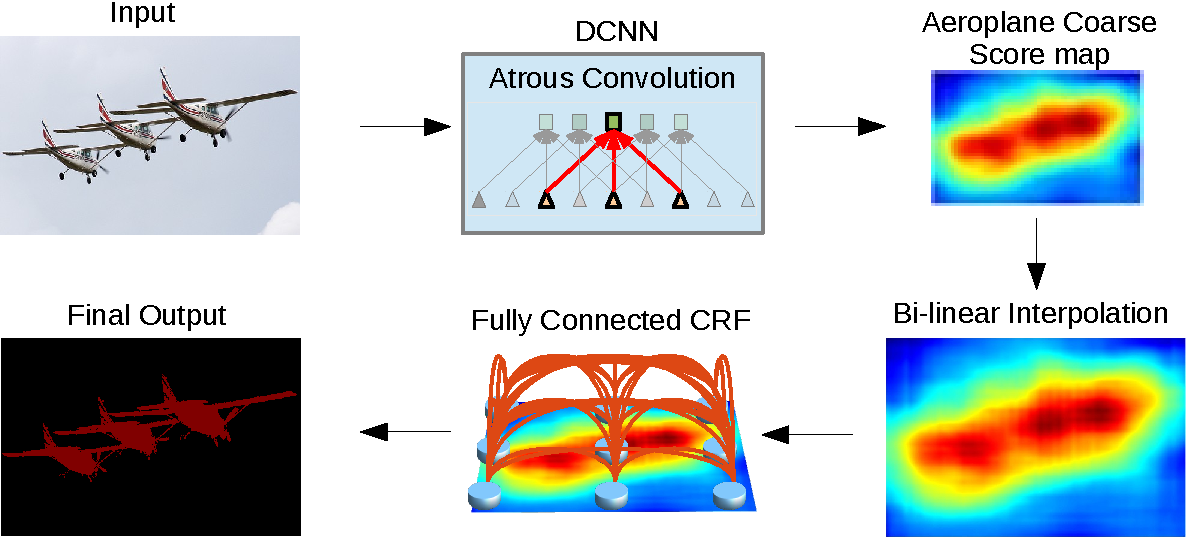
\includegraphics[width=0.7\linewidth]{fig/model_illustration4.pdf}
  \caption{模型图。诸如 VGG-16 或 ResNet-101 之类的 DCNNs 以完全卷积的方式使用,使用空洞卷积来降低信号下采样的程度(从32$\times$ 下降到 8$\times$)。双线性插值将特征放大到原始图像分辨率。然后使用完全连接的 CRF 来细化分割结并更好地捕获物体边界。} \label{fig:ModelIllustration}
\end{figure*}

\figref{fig:ModelIllustration} 展示了我们提出的 DeepLab 模型的高层结构。在图像分类任务中训练的深度卷积网络(VGG-16 \cite{simonyan2014very} 或 ResNet-101 \cite{he2015deep})通过以下方式重新运用于图像语义分割任务:(1)将所有全连接层换成卷积层 \cite{long2014fully},(2)通过空洞卷积层增加特征分辨率,使得我们能计算原图中每8个像素的特征而不是每32个。然后,我们采用双线性插值将分类分数图上采样 8 倍,以达到原图分辨率,从而产生全连接 CRF 的输入 \cite{krahenbuhl2011efficient},来达到细化分割结果的目的。

从实用的角度来看,我们的 DeepLab 系统有三大优点:(1)速度:由于空洞卷积的使用,我们的 DCNN 以 8 FPS 的速度在 NVidia Titan X GPU 上运行,全连接 CRF 的平均场推断在 CPU 上需要大约 0.5 秒;(2)精度:在众多图像分割数据集挑战中,我们的模型一举夺魁,包括 PASCAL VOC 2012 \cite{everingham2014pascal}, PASCAL-Context \cite{mottaghi2014role}, PASCAL-Person-Part \cite{chen_cvpr14} 以及 Cityscapes \cite{Cordts2016Cityscapes};(3)复杂度:我们的系统是由 DCNNs 和 CRFs 这两个非常成熟的模块级联组合而成的,便于理解和编写。

这篇论文中介绍的更新过的 DeepLab 与我们最初发表的第一个版本相比有几项改进 \cite{chen2014semantic}。新版本能够通过多尺度输入 \cite{farabet2013learning, lin2015efficient, chen2015attention} 或 ASPP 更好地分割多个尺度下的物体。我们通过调整最新的 ResNet \cite{he2015deep} 图像分类 DCNN 构建了 DeepLab 的残差网络变体,与基于 VGG-16 \cite{simonyan2014very} 的原始模型相比,拥有更优的语义分割性能。最后,我们对多种模型变体进行了更全面的实验评估,并报告了最新结果,不仅是 PASCAL VOC 2012,还有其他具有挑战性的任务。我们通过扩展 Caffe 框架 \cite{jia2014caffe} 实现了 DeepLab,并在 \url{http://liangchiehchen.com/projects/DeepLab.html} 开放了源代码及模型数据。

\section{Related Work}

过去十年里,大多数成功的语义分割系统都依赖于人工特征与平面分类器的结合,例如 Boosting \cite{TuB10,shotton2009textonboost}, 随机森林 \cite{shotton2008semantic}, 支持向量机 \cite{FulkersonVS09}。通过结合来自上下文 \cite{carreira2012semantic} 和结构化预测技术 \cite{he2004multiscale,ladicky2009associative,carreira2012cpmc,krahenbuhl2011efficient} 的更丰富的信息,语义分割系统已经实现了实质性的改进,但是这些系统的性能一直受到特征的有限表现能力的约束。在过去几年里,深度学习在计算机视觉方向上的突破从图像分类很快转移到了语义分割。由于这个任务涉及到边界分割与物体分类,因此,其核心问题在于如何组合这两个子任务。

用于语义分割的第一类基于 DCNN 的系统通常采用自下而上的图像分割级联,然后再对划分区域使用 DCNN 进行分类。例如,边界框和被其框住的区域 \cite{arbelaez2014multiscale, Uijlings13} 被同时输入给 DCNN 用于区域分类 \cite{girshick2014rcnn, hariharan2014simultaneous},以将形状信息结合到分类过程中。类似地,\cite{mostajabi2014feedforward} 的作者靠的是图片的超像素表达。尽管这些方法可以从良好分割所带来的明显边界中受益,但它们也无法从其任何错误中恢复。

第二类依赖于使用卷积计算的 DCNN 特征进行密集图像标记,并与独立获得的分割结合起来。首先是 \cite{farabet2013learning} 以多重分辨率使用 DCNN,然后使用分割树来平滑化分类结果。最近,\cite{hariharan2014hypercolumns} 提出使用跳跃层并连接 DCNN 中计算出的特征以进行像素分类。此外,\cite{dai2014convolutional} 提出利用候选区域集合计算特征图。这些工作仍采用与DCNN 分类器结果分离的分段算法,因此有可能导致过早的决策。

第三类直接使用 DCNN 进行密集的像素级分类,这样能避免分段决策。\cite{long2014fully, eigen2014predicting} 的无分段方法以完全卷积的方式直接将 DCNN 应用于整个图像,将 DCNN 的最后全连接层转换为卷积层。为了处理引言中提到的空间定位问题,\cite{long2014fully} 对特征的得分图进行上采样和连接,而 \cite{eigen2014predicting} 通过将粗略结果传给另一个 DCNN,从而细化预测结果。我们的工作建立在这些工作的基础上,并且如引言中所述通过控制特征分辨率来扩展它们,引入多尺度池化技术并将全连接的 CRF \cite{krahenbuhl2011efficient} 集成在 DCNN 之上。我们发现这会导致明显更好的分割结果,尤其是沿着物体边界。DCNN 与 CRF 的组合使用并非史无前例,但是已有的研究工作中仅仅尝试了 locally-connected 的 CRF 模型。具体而言,\cite{cogswell2014combining} 使用 CRFs 作为基于 DCNN 的重排序系统的建议方法,\cite{farabet2013learning} 将超像素看做是本地成对 CRF 的节点,并使用图形分割进行离散推理。因此,他们的模型受到超像素计算中的错误或忽略的长远依赖的限制。然而,我们的方法将每个像素视为由 DCNN 接收的唯一的 CRF 节点。值得强调的是,我们采用的全连接 CRF 模型使用高斯 CRF 捕捉长远依赖关系 \cite{krahenbuhl2011efficient},同时,这个模型也适用于快速平均场推断。我们注意到,对于传统的图像分割任务,\cite{geiger1991parallel, geiger1991common, kokkinos2008computational} 已经广泛研究了平均场推断方法,但这些老旧的模型通常仅限于短程连接,难以捕获长程关系。在独立工作中, \cite{bell2014material} 使用非常类似于密集连接的 CRF 模型来细化针对材料分类问题的 DCNN 的结果。然而,\cite{bell2014material} 的 DCNN 模块仅通过稀疏点监督训练,而不是每个像素。

由于本研究工作的初代版本已公开发布 \cite{chen2014semantic},图像语义分割领域已经取得了巨大的进展。多个研究小组都有着重大的突破进展,显著地提高了 PASCAL VOC 2012 的基线,这也反映了基准测试排行榜\footnote{\url{http://host.robots.ox.ac.uk:8080/leaderboard/displaylb.php?challengeid=11&compid=6}} \cite{papandreou2015weakly, zheng2015conditional, dai2015boxsup, noh2015learning, liu2015semantic, lin2015efficient, chen2015attention, chen2015semantic}上水平之高。有趣的是,大多数表现最佳的方法都采用了我们 DeepLab 系统的一两个关键要素:(1)通过空洞卷积进行高效密集特征提取和(2)通过全连接 CRF 对原始DCNN分数的细化。我们在下面概述了一些最重要、最有趣的进展。

\newcommand{\mycomment}[1]{}
\mycomment{
	A key difference compared to \cite{long2014fully} lies in the way we produce
	feature maps at the original image resolution: They use a sequence of
	deconvolutional layers \cite{zeiler2014visualizing}, while we use a combination
	of atrous convolution and bilinear interpolation, resulting in a significantly
	simpler system that explicitly handles the signal downsampling issue, requires
	fewer parameters, and is easier to train.
}

大量相关工作中使用了 \textit{端到端训练结构化预测} 的方法。虽然我们使用 CRF 作为后处理方法,但在 \cite{zheng2015conditional, chen2014learning, schwing2015fully, liu2015semantic, lin2015efficient} 中,研究者已经成功地进行了 DCNN 与 CRF 的联合学习。特别是 \cite{zheng2015conditional, schwing2015fully} 展开了 CRF 的平均场推断,将整个系统转化为可端到端训练的前馈网络,而 \cite{liu2015semantic} 使用带有可学习滤波器的卷积层近似了密集 CRF 一轮平均场推断迭代 \cite{krahenbuhl2011efficient}。\cite{lin2015efficient, chandra2016fast} 使用 DCNN 学习 CRF 的成对点关系,它以繁重的计算为代价提升了模型的准度。\cite{chen2015semantic} 使用更快的域变换模块 \cite{GastalOliveira2011DomainTransform} 替换平均场推断中的双边滤波模块,以提升运算速度降低内存占用。而 \cite{bertasius2015high, kokkinos2016pushing} 将语义分割与边缘检测算法结合起来。

许多论文中使用了 \textit{弱监督训练},放宽了像素级语义注释可用于整个训练集的假设 \cite{pinheiro2014weakly, papandreou2015weakly, pathakICCV15ccnn, hong2015decoupled},取得了比弱监督训练 pre-DCNN 更好的结果 \cite{vezhnevets2011weakly}。在另一个研究领域,\cite{hariharan2014simultaneous, liang2015proposal} 追求实例细分,共同解决对象检测和语义分割。

我们称为 \textit{空洞卷积} 的技术源于计算小波变换的 ``algorithme \`a trous'' \cite{holschneider1989real}。我们建议感兴趣的读者朋友引用 \cite{fowler2005redundant} 来获得小波变换的早期文献资料。空洞卷积也与多速率信号处理中的 ``noble identities'' 密切相关,它也是基于输入信号与滤波器采样率的函数 \cite{vaidyanathan1990multirate}。空洞卷积概念是我们在 \cite{papandreou2014untangling} 中首次提出的。同样的操作后来被称之为 \textit{扩张卷积} \cite{yu2015multi},基于对应操作中包含上采样(\cite{holschneider1989real} 也称为 扩张)这一事实。为了在 DCNNs 中获取更为密集的特征,许多研究者也曾使用过相同的操作 \cite{giusti2013fast, sermanet2013overfeat, papandreou2014untangling}。除了提升分辨率之外,空洞卷积允许我们扩大滤波器的感受野以包含更大的上下文,我们在 \cite{chen2014semantic} 中发现这是有益的。这种方法已被 \cite{yu2015multi} 进一步提升,他使用一系列空洞卷积层来聚合多尺度上下文。我们提出的用于捕获多尺度物体和上下文的空洞空间金字塔池化方法也采用具有不同采样率的多个空洞卷积层,但是,我们是并行而非串行使用。有趣的是,空洞卷积也被运用于更广泛的任务,例如物体检测 \cite{liu2015ssd,dai2016rfcn}、实例分割 \cite{dai2016instance}、视觉问答 \cite{chen2015abc}、光流系统 \cite{sevilla2016optical} 等。

我们还表明,正如预期所料,集成到 DeepLab 中的更高级的图像分类 DCNNs 可以带来更好的结果(如 \cite{he2015deep} 的 ResNet), \cite{wu2016high} 也观察到了这一点。

\section{Methods}
\label{sec:methods}

\subsection{Atrous Convolution for Dense Feature Extraction and Field-of-View Enlargement}
\label{sec:convnet-hole}
The use of DCNNs for semantic segmentation, or other dense prediction tasks, has been shown to be
simply and successfully addressed by deploying DCNNs in a fully convolutional fashion \cite{sermanet2013overfeat, long2014fully}.
 However, the repeated combination of max-pooling and striding
 at consecutive layers of these networks reduces significantly the spatial resolution of the
 resulting feature maps, typically by a factor of 32 across each direction in recent DCNNs.
 A partial remedy is to use `deconvolutional' layers as  in  \cite{long2014fully},
which however requires additional memory and time.
 
We advocate instead the use of atrous convolution, originally developed for the efficient computation of the
undecimated wavelet transform in the ``algorithme \`a trous'' scheme of
\cite{holschneider1989real} and used before in the DCNN context by
\cite{giusti2013fast, sermanet2013overfeat, papandreou2014untangling}.
This algorithm allows us to compute the responses of any layer at any desirable resolution.
It can be applied post-hoc, once a network has been trained, but can also be seamlessly integrated with training.

Considering one-dimensional signals first, the output $y[i]$ of atrous convolution \footnote{We follow the
standard practice in the DCNN literature and use non-mirrored filters in this
definition.} of a 1-D input signal $x[i]$ with a filter $w[k]$ of length $K$ is
defined as:
\begin{equation}
  y[i] = \sum_{k=1}^K x[i + r \cdot k] w[k].
\end{equation}
The \emph{rate} parameter $r$ corresponds to the stride with which we sample the
input signal. Standard convolution is a special case for rate $r = 1$.
See \figref{fig:hole} for illustration.

 \begin{figure}
  \begin{tabular}{c}
%  \includegraphics[width=0.5\linewidth]{fig/atrous2.pdf}
    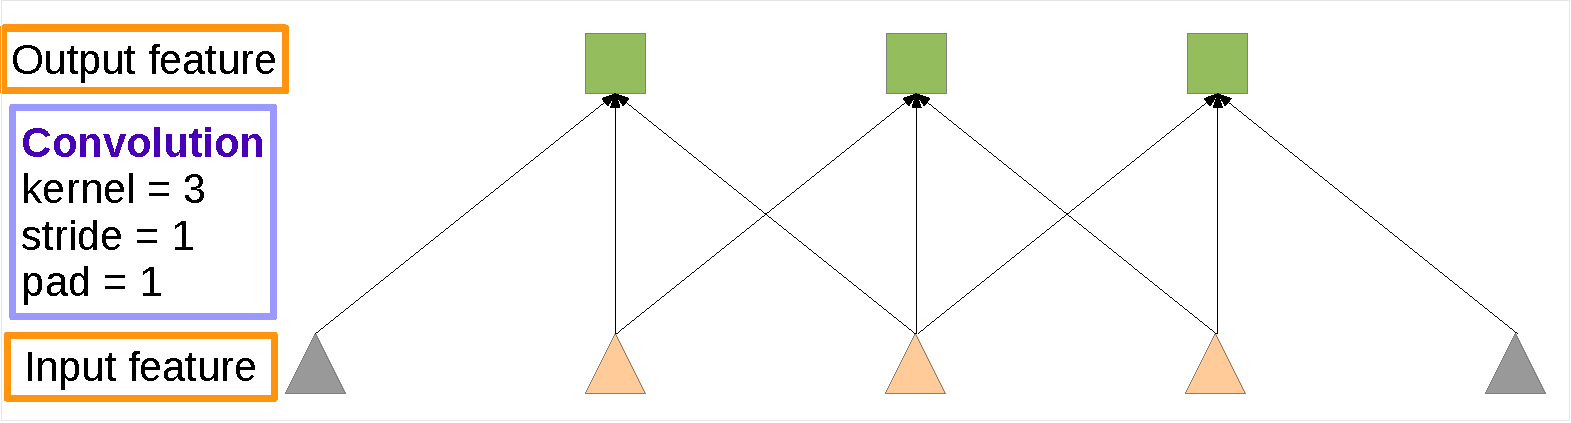
\includegraphics[width=0.9\linewidth]{fig/atrous_fig1.pdf} \\
    {\scriptsize (a) Sparse feature extraction} \\
    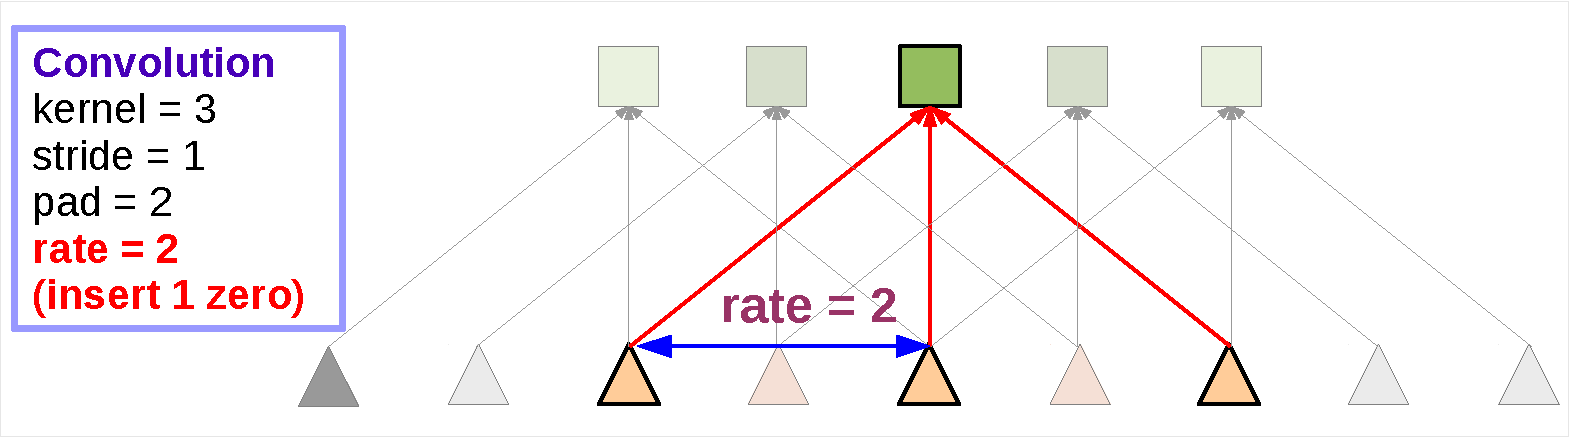
\includegraphics[width=0.9\linewidth]{fig/atrous_fig2.pdf} \\
    {\scriptsize (b) Dense feature extraction} \\
  \end{tabular}
  \caption{Illustration of atrous convolution in 1-D. (a) Sparse feature
    extraction with standard convolution on a low resolution input feature map.
    (b) Dense feature extraction with atrous convolution with rate $r = 2$,
    applied on a high resolution input feature map.}
  \label{fig:hole}
\end{figure}

We illustrate the algorithm's operation in 2-D through a simple example in \figref{fig:hole2d}: Given an image, we 
assume that we first have a downsampling operation that reduces the resolution by a factor of 2, and then perform  a 
convolution with a  kernel - here, the vertical Gaussian derivative. If one  implants the resulting 
feature map in the original image coordinates, we realize that we have obtained responses at only 1/4 of the image positions. 
Instead, we can compute responses at all image positions 
if we convolve the full resolution image with a filter `with holes', in which 
we upsample the original filter by a
factor of 2, and introduce zeros  in between filter values. 
Although the effective filter size increases, we only need to take into account the
non-zero filter values, hence both the number of filter parameters and the number of operations per position stay constant. 
The resulting scheme allows us to easily and explicitly control the spatial resolution of neural
network feature responses.

\begin{figure}
  \centering
    \begin{tabular}{c}
    	%  \includegraphics[width=0.5\linewidth]{fig/atrous2.pdf}
    	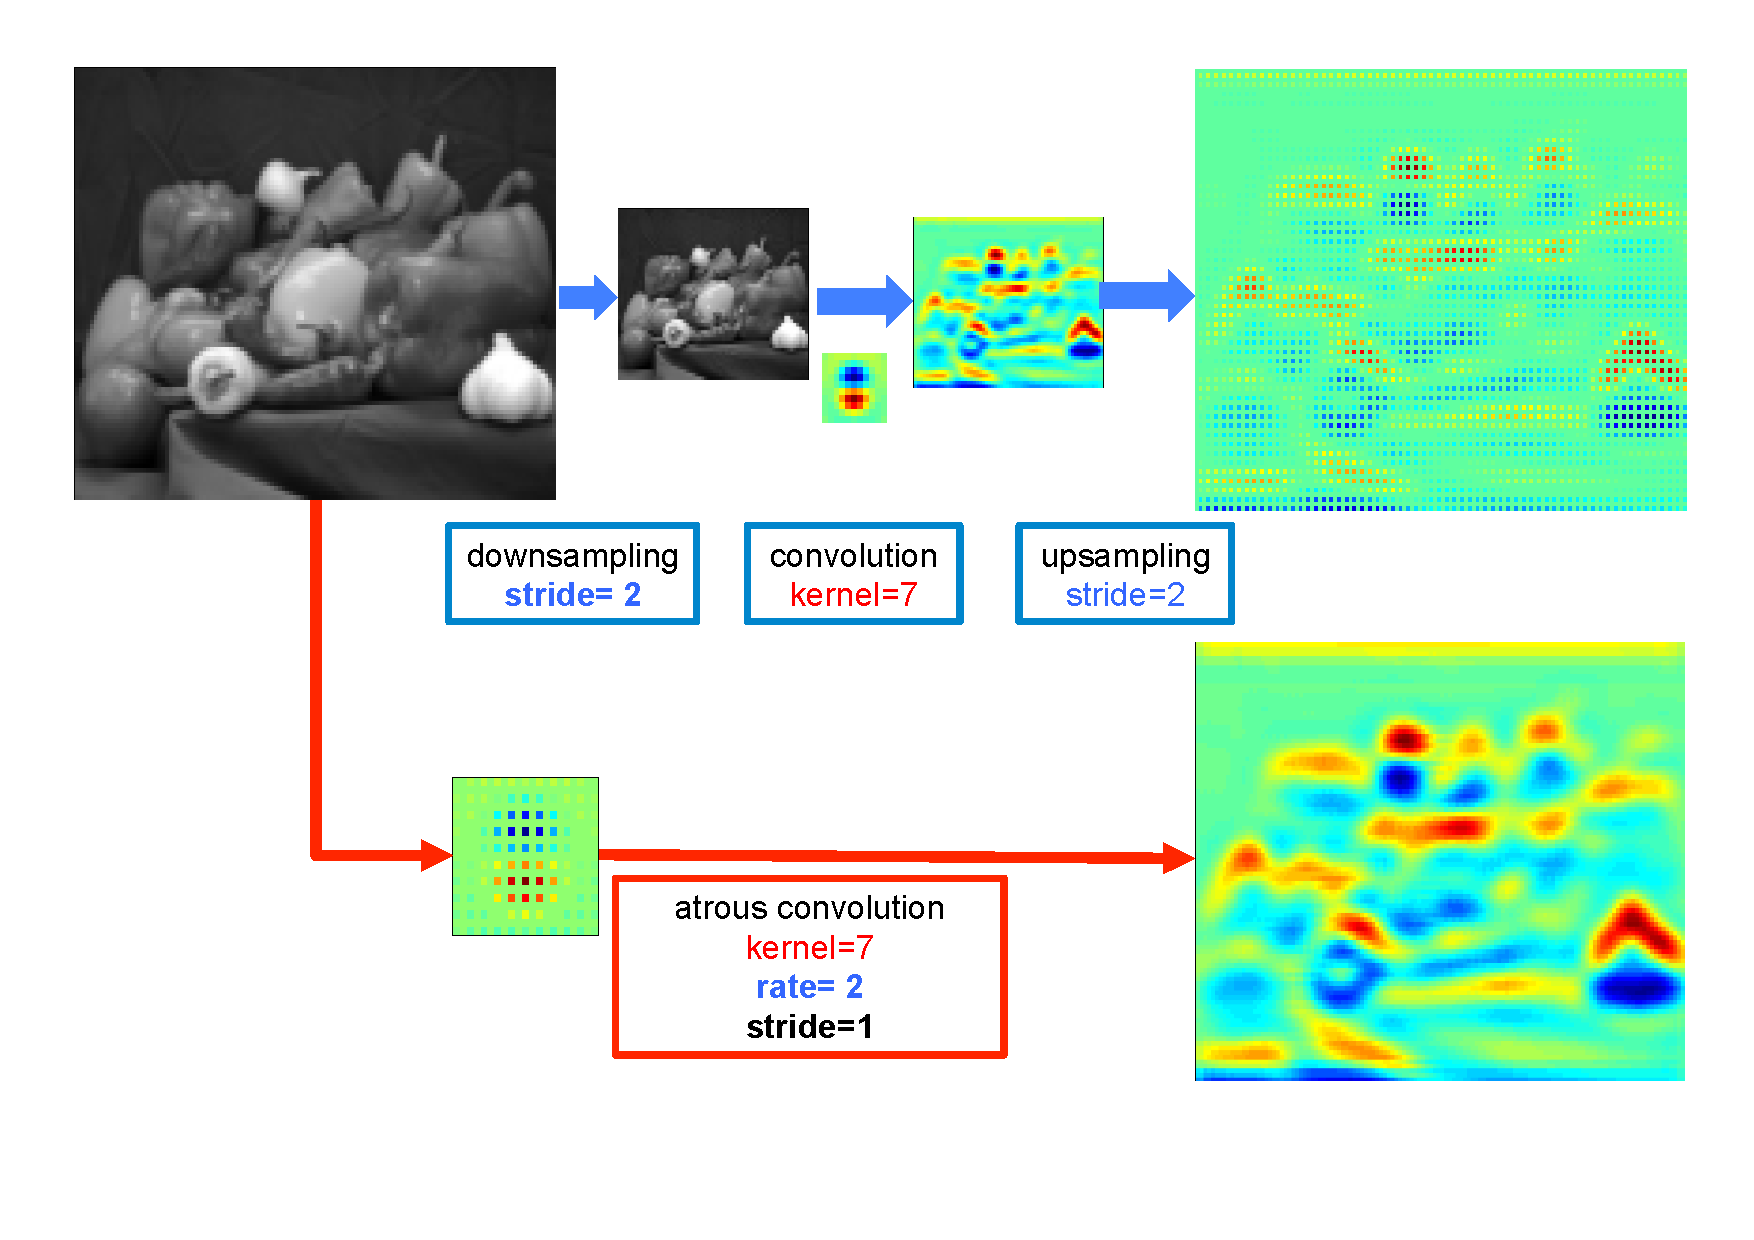
\includegraphics[width=.99 \linewidth]{fig/atrous_slide_rate.pdf}
    	\vspace{-.9cm}
    \end{tabular}
   \caption{Illustration of atrous convolution in 2-D. Top row: sparse feature
   	extraction with standard convolution on a low resolution input feature map.
   	Bottom row: Dense feature extraction with atrous convolution with rate $r = 2$,
   	applied on a high resolution input feature map.}
    \label{fig:hole2d}
   \end{figure}

In the context of DCNNs one can use  atrous convolution in a chain of layers,
 effectively allowing us to compute the final DCNN network responses at an
arbitrarily high resolution. For example, in order to double the spatial density
of computed feature responses in the VGG-16 or ResNet-101 networks, we find the
last pooling or convolutional layer that decreases resolution ('pool5' or 'conv5\_1'
respectively), set its stride to 1 to avoid signal decimation, and replace all
subsequent convolutional layers with atrous convolutional layers having rate
$r = 2$. 
Pushing this approach all the
way through the network could allow us to compute feature responses at the original image
resolution, but this ends up being too
costly. We have adopted instead a hybrid approach that strikes a
good efficiency/accuracy trade-off, using atrous convolution to increase by a
factor of 4 the density of computed feature maps, followed by fast bilinear
interpolation by an additional factor of 8 to
recover feature maps at the original image resolution. Bilinear interpolation
is sufficient in this setting because the class score maps (corresponding to
log-probabilities) are quite smooth, as illustrated in
\figref{fig:score-maps}. Unlike the deconvolutional approach adopted by
\cite{long2014fully}, the proposed approach converts image classification
networks into dense feature extractors without requiring learning any extra
parameters, leading to faster DCNN training in practice. 

Atrous convolution also allows us to arbitrarily enlarge the \emph{field-of-view} of
filters at any DCNN layer.
State-of-the-art DCNNs typically employ spatially small
convolution kernels (typically \by{3}{3}) in order to keep both computation and
number of parameters contained. Atrous convolution with rate $r$ introduces
$r-1$ zeros between consecutive filter values, effectively enlarging the kernel
size of a \by{k}{k} filter to $k_e = k + (k-1)(r-1)$ without increasing the
number of parameters or the amount of computation. It thus offers an efficient
mechanism to control the field-of-view and finds the best trade-off between
accurate localization (small field-of-view) and context assimilation (large
field-of-view). We have successfully experimented with this technique:
Our DeepLab-LargeFOV model variant \cite{chen2014semantic} employs atrous
convolution with rate $r = 12$ in VGG-16 `fc6' layer with significant
performance gains, as detailed in Section~\ref{sec:experiments}.

Turning to implementation aspects, 
there are two efficient ways to  perform atrous convolution. The first
is to implicitly upsample the filters by inserting holes (zeros), or
equivalently sparsely sample the input feature maps \cite{holschneider1989real}.
We implemented this in our earlier work \cite{papandreou2014untangling,
 chen2014semantic}, followed by \cite{yu2015multi}, within the Caffe framework
\cite{jia2014caffe} by adding to the \textsl{im2col} function (it extracts
vectorized patches from multi-channel feature maps) the option to sparsely
sample the underlying feature maps. The second method, originally proposed by
\cite{shensa1992discrete} and used in \cite{giusti2013fast, sermanet2013overfeat}
is to subsample the input feature map by a factor equal to the atrous
convolution rate $r$, deinterlacing it to produce $r^2$ reduced resolution maps,
one for each of the $\by{r}{r}$ possible shifts. This is followed by applying
standard convolution to these intermediate feature maps and reinterlacing them
to the original image resolution. By reducing atrous convolution into regular
convolution, it allows us to use off-the-shelf highly optimized convolution
routines. We have implemented the second approach into the TensorFlow framework
\cite{abadi2016tensorflow}.

%% When applying networks designed for image classification in a fully
%% convolutional fashion for dense prediction tasks, one converts the last fully
%% connected layers into convolutional ones \cite{long2014fully}. This implies
%% that the network spends a much larger fraction of computation in its last
%% few layers, making them the computational bottleneck during both training
%% and evaluation. We have found that we can significantly accelerate a fully
%% convolutional version of the VGG-16 network and at the same time reduce its
%% memory footprint by making two key changes: (1) Thinning the activation maps
%% in the last two hidden layers by a factor of 4, by retaining a random subset
%% of 1,024 out of the original 4,096 filters. (2) Reducing the filter size of
%% the first fully connected layer down to \by{3}{3} (or \by{4}{4}) by
%% subsampling the original \by{7}{7} filters. These changes significantly
%% increase the computational efficiency of our model.

\subsection{Multiscale Image Representations using Atrous Spatial Pyramid Pooling}

DCNNs have shown a remarkable
ability to implicitly represent scale, simply by being trained on datasets that
contain objects of varying size. Still, explicitly accounting for object scale
can improve the DCNN's ability to successfully handle both
large and small objects \cite{papandreou2014untangling}.

We have experimented with two approaches to handling
 scale variability in semantic segmentation.
The first approach amounts to standard multiscale
processing \cite{chen2015attention, kokkinos2016pushing}. We extract DCNN score
maps from multiple (three in our experiments) rescaled versions of the original
image using parallel DCNN branches that share the same parameters. To produce
the final result, we bilinearly interpolate the feature maps from the parallel
DCNN branches to the original image resolution and fuse them, by taking at each
position the maximum response across the different scales. We do this both
during training and testing. Multiscale processing significantly improves
performance, but at the cost of computing feature responses at all DCNN layers for
multiple scales of input. 

The second approach is inspired by the success of the R-CNN spatial pyramid pooling method of \cite{he2014spatial},
which showed that regions of an arbitrary scale can be accurately and efficiently classified by resampling 
convolutional features extracted at a single scale.
 We have implemented a variant of their scheme which uses multiple
parallel atrous convolutional layers with different sampling rates. The features extracted for each sampling
rate are further processed in separate branches and fused to generate the final
result. The proposed ``atrous spatial pyramid pooling'' (DeepLab-ASPP) approach
generalizes our DeepLab-LargeFOV variant and is illustrated in \figref{fig:aspp_fov}.

%%  for the VGG-16 network, where ASPP is applied to the `pool5' features,
%% delivering the input to layer `fc6'.
%%  Another related approach has been successfully pursued by \cite{yu2015multi}: they
%% employ a cascade of serially connected atrous convolutional layers with
%% increasing rate parameters on top of the class score maps, which they show to be
%% effective at capturing multiscale context.

\begin{figure}[!t]
  \centering
  \scalebox{1}{
  \begin{tabular}{c}
    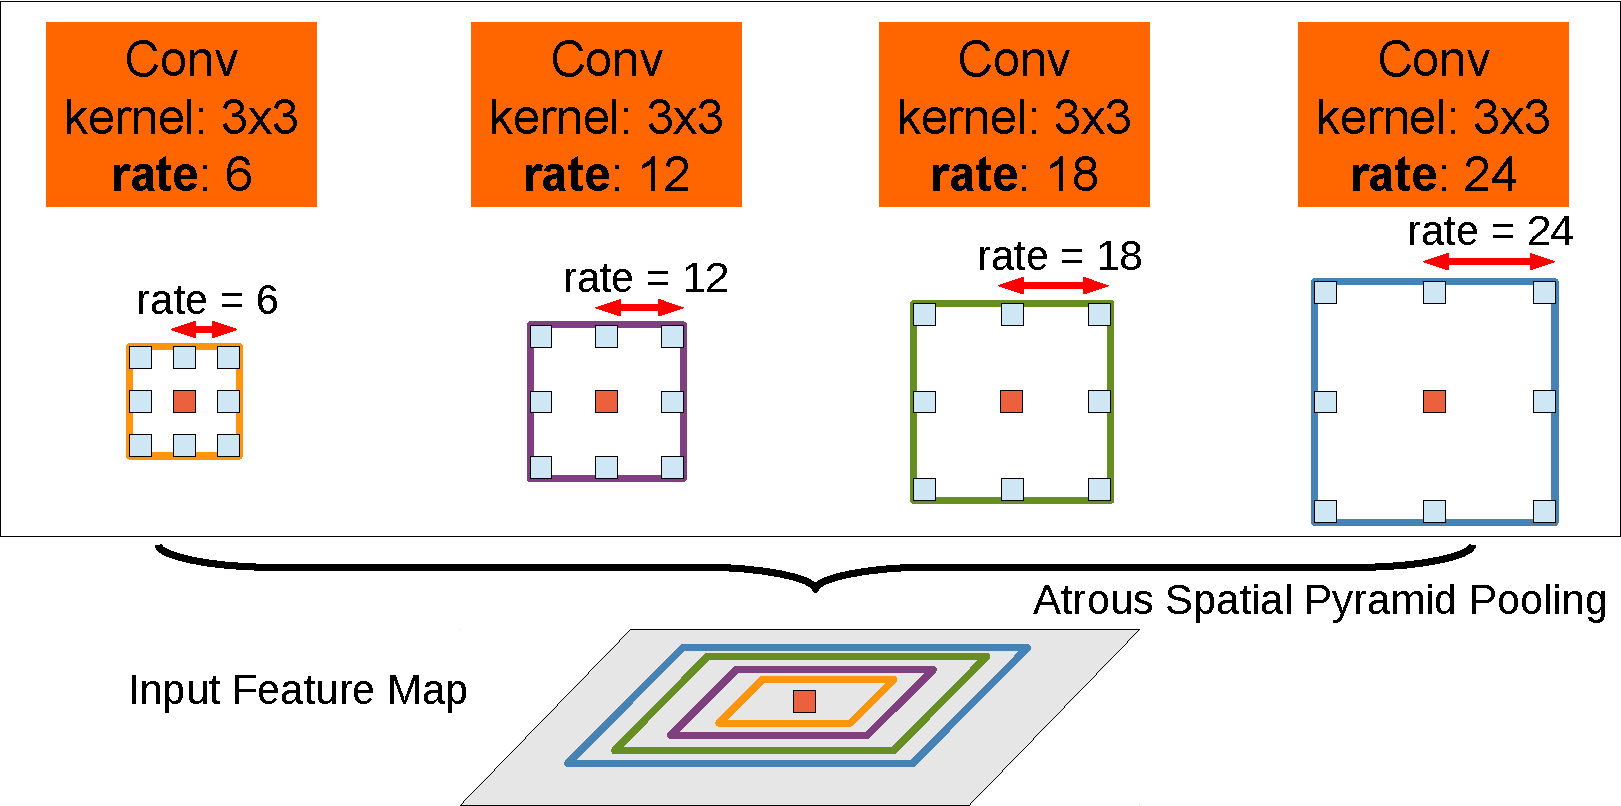
\includegraphics[height=4.5cm]{./fig/spm/aspp2.pdf} \\
  \end{tabular}
  }
  \caption{Atrous Spatial Pyramid Pooling (ASPP). To classify the center pixel (orange),
    ASPP exploits multi-scale features by employing multiple parallel filters with
    different rates. The effective Field-Of-Views are shown in different colors.}
  \label{fig:aspp_fov}
\end{figure}

\subsection{Structured Prediction with Fully-Connected Conditional Random Fields for Accurate Boundary Recovery}
\label{sec:boundary-recovery}

A trade-off between localization accuracy and classification performance seems to be inherent in DCNNs:
deeper models with multiple max-pooling layers have
proven most successful in classification tasks, however the increased
invariance and the large receptive fields of top-level nodes can only yield smooth responses.
%\label{sec:local-chal}
As illustrated in \figref{fig:score-maps}, DCNN score maps can
 predict the presence and rough position of objects but
cannot really delineate their borders. 

Previous work has pursued two directions to address this localization challenge.
The first approach is to harness information from multiple layers in the
convolutional network in order to better estimate the object boundaries
\cite{hariharan2014hypercolumns, long2014fully, eigen2014predicting}. The
second  is to employ a super-pixel representation, essentially
delegating the localization task to a low-level segmentation method
\cite{mostajabi2014feedforward}.

%We have also
%pursued a hybrid approach in which we combine the proposed fully-connected CRF
%method with our own variant of multi-scale prediction. This combined approach
%yields a further performance improvement, as discussed in
%Section~\ref{sec:multiscale}.

%\textbf{Fully-Connected Conditional Random Fields for Accurate Localization}
%\label{sec:dense-crf}

We pursue an alternative direction based on coupling the recognition
capacity of DCNNs and the fine-grained localization accuracy of fully connected
CRFs and show that it is remarkably successful in addressing the localization
challenge, producing accurate semantic segmentation results and recovering
object boundaries at a level of detail that is well beyond the reach of existing
methods. This direction has been extended by several follow-up papers
\cite{papandreou2015weakly, schwing2015fully, zheng2015conditional,
  dai2015boxsup, noh2015learning, liu2015semantic, lin2015efficient,
  chen2015attention, chen2015semantic}, since the first version of our work
was published \cite{chen2014semantic}.

\begin{figure}[t]
  \centering
  \begin{tabular}{c c c c c}
    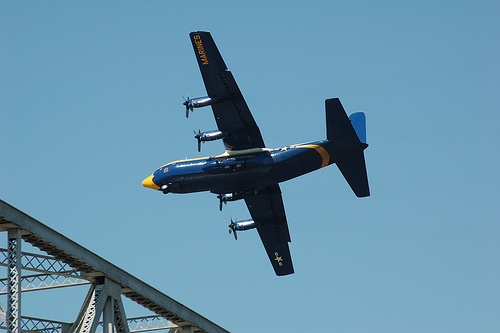
\includegraphics[width=0.16\linewidth]{fig/mean_field_illustration/2007_007470.jpg} & 
    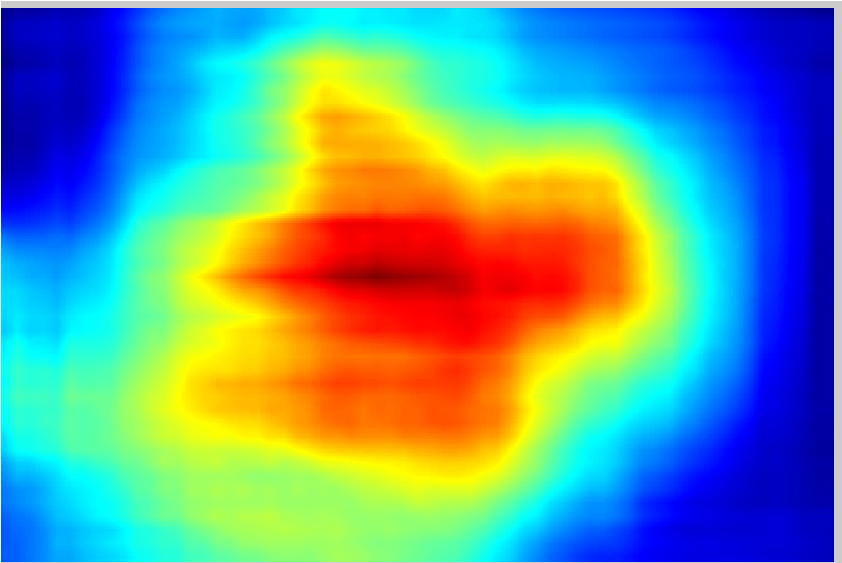
\includegraphics[width=0.16\linewidth]{fig/mean_field_illustration/Score_Class1_Itr0.pdf} &
    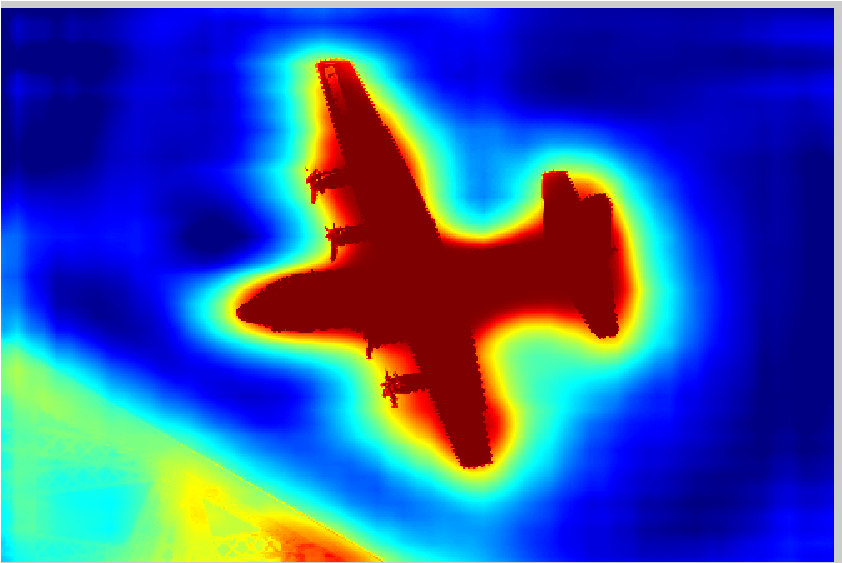
\includegraphics[width=0.16\linewidth]{fig/mean_field_illustration/Score_Class1_Itr1.pdf} & 
    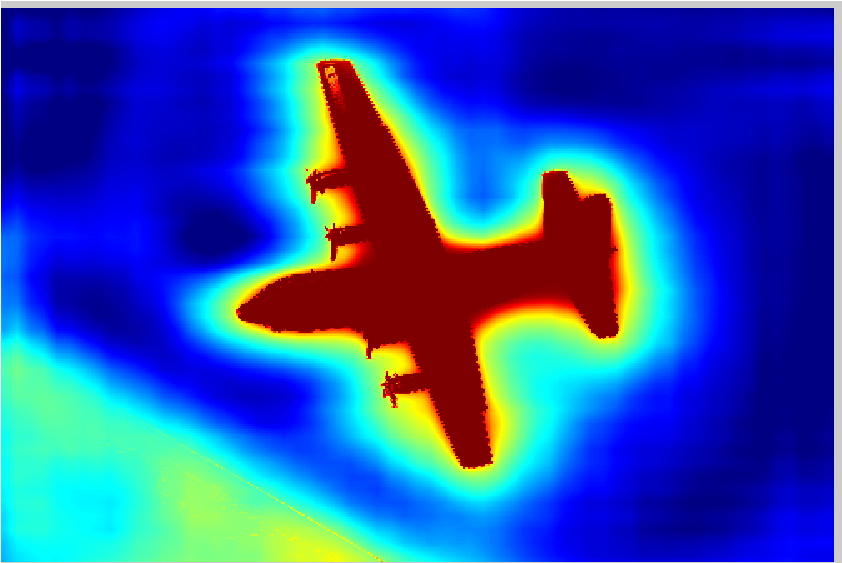
\includegraphics[width=0.16\linewidth]{fig/mean_field_illustration/Score_Class1_Itr2.pdf} & 
    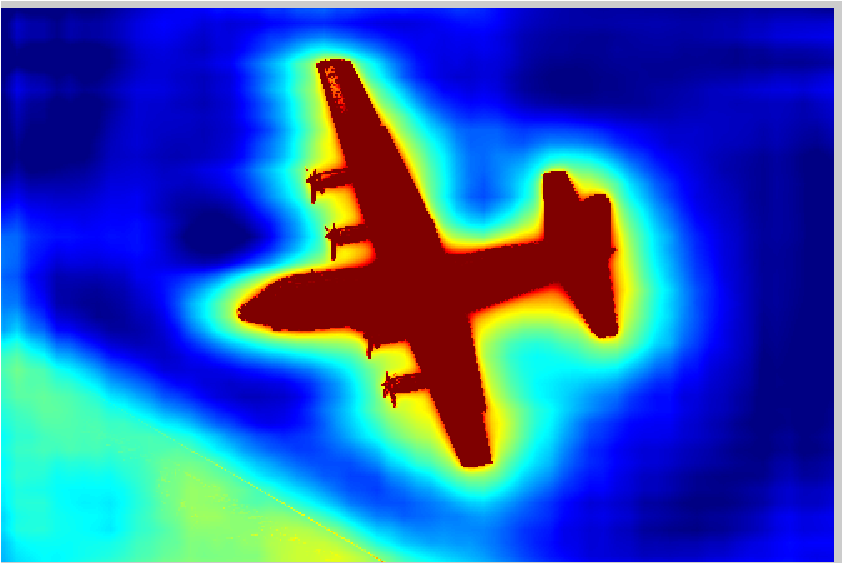
\includegraphics[width=0.16\linewidth]{fig/mean_field_illustration/Score_Class1_Itr10.pdf} \\
    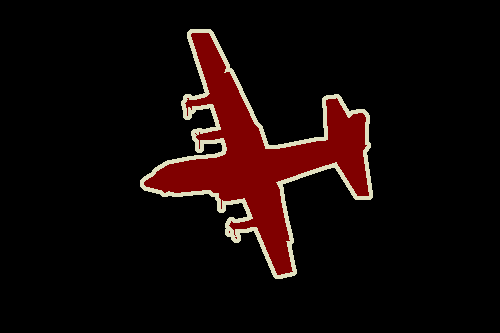
\includegraphics[width=0.16\linewidth]{fig/mean_field_illustration/2007_007470.png} & 
    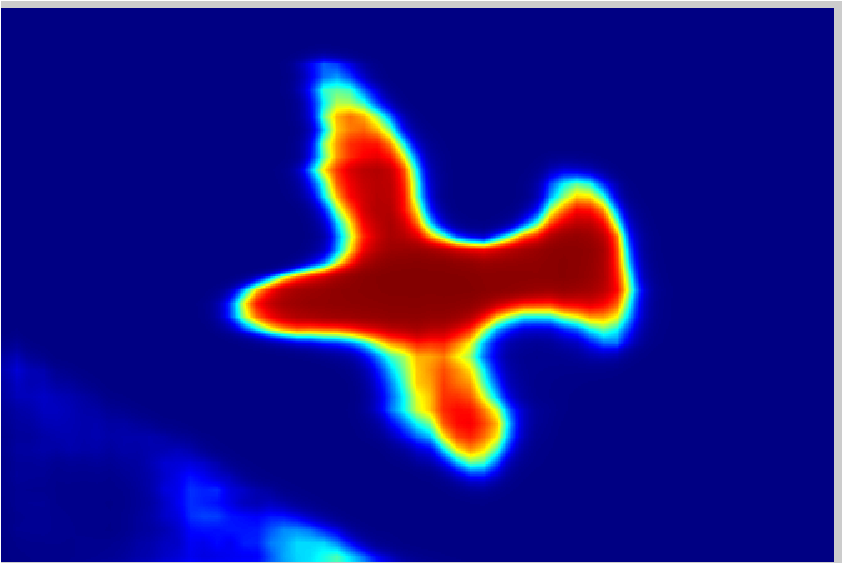
\includegraphics[width=0.16\linewidth]{fig/mean_field_illustration/Belief_Class1_Itr0.pdf} & 
    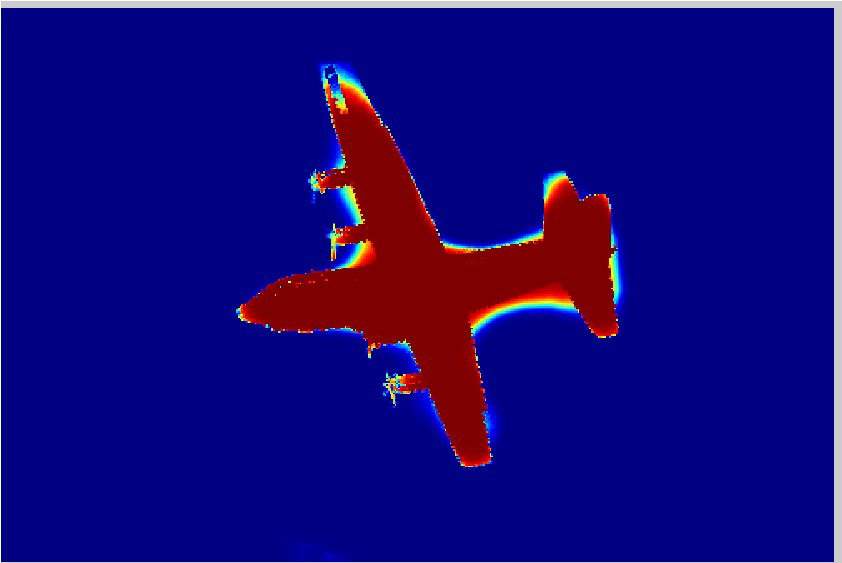
\includegraphics[width=0.16\linewidth]{fig/mean_field_illustration/Belief_Class1_Itr1.pdf} & 
    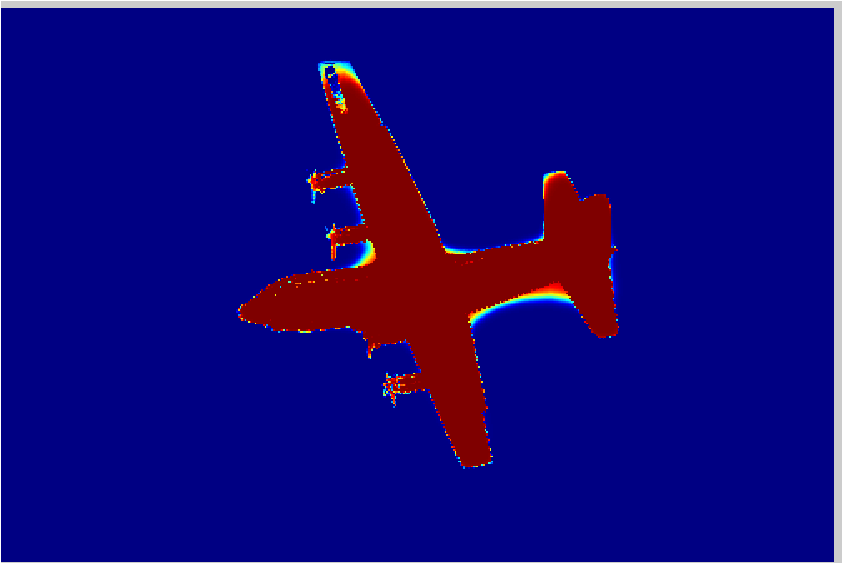
\includegraphics[width=0.16\linewidth]{fig/mean_field_illustration/Belief_Class1_Itr2.pdf} & 
    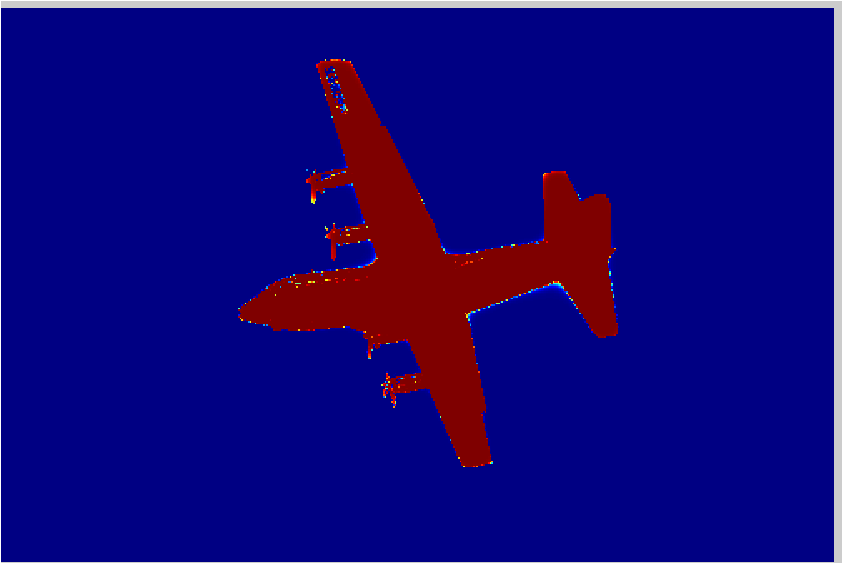
\includegraphics[width=0.16\linewidth]{fig/mean_field_illustration/Belief_Class1_Itr10.pdf} \\
    {\tiny Image/G.T.} & {\tiny DCNN output} & {\tiny CRF Iteration 1} & {\tiny CRF Iteration 2} & {\tiny CRF Iteration 10} \\
  \end{tabular}
  \caption{Score map (input before softmax function) and belief map (output of
    softmax function) for Aeroplane. We show the score (1st row) and belief (2nd row)
    maps after each mean field iteration. The output of last DCNN layer is used as
    input to the mean field inference.}
  \label{fig:score-maps}
\end{figure}

Traditionally, conditional random fields (CRFs) have been employed to smooth
noisy segmentation maps \cite{rother2004grabcut, kohli2009robust}. Typically
these models  couple neighboring nodes, favoring
same-label assignments to spatially proximal pixels. Qualitatively, the
primary function of these short-range CRFs is to clean up the spurious
predictions of weak classifiers built on top of local hand-engineered features.

Compared to these weaker classifiers, modern DCNN architectures such as
the one we use in this work produce score maps and semantic label
predictions which are qualitatively different. As illustrated in
\figref{fig:score-maps}, the score maps are typically quite smooth and
produce homogeneous classification results. In this regime, using short-range
CRFs can be detrimental, as our goal should be to recover detailed local
structure rather than further smooth it. Using contrast-sensitive potentials
\cite{rother2004grabcut} in conjunction to local-range CRFs can potentially
improve localization but still miss thin-structures and typically requires
solving an expensive discrete optimization problem.

To overcome these limitations of short-range CRFs, we integrate into our system
the fully connected CRF model of \cite{krahenbuhl2011efficient}. The model
employs the energy function
\begin{align}
  E(\boldsymbol{x}) = \sum_i \theta_i(x_i) + \sum_{ij} \theta_{ij}(x_i, x_j)
\end{align}
where $\boldsymbol{x}$ is the label assignment for pixels. We use as unary
potential $\theta_i(x_i) = - \log P(x_i)$, where $P(x_i)$ is the label
assignment probability at pixel $i$ as computed by a DCNN. The pairwise
potential has a form that allows for efficient inference while using a fully-connected graph, i.e.
when  connecting 
all pairs of image pixels, $i,j$. In particular, as in \cite{krahenbuhl2011efficient},  we use the following expression:
\begin{gather}
 \hspace{-.2cm}\theta_{ij}(x_i, x_j) \!=\! \mu(x_i,x_j)\!\left[w_1 \exp \Big(\!-\!\frac{||p_i-p_j||^2}{2\sigma_\alpha^2} \!-\!\frac{||I_i-I_j||^2}{2\sigma_\beta^2}\! \Big)\right. \nonumber\\
\left. + w_2 \exp \Big(-\frac{||p_i-p_j||^2}{2\sigma_\gamma^2}\Big)\right]\label{eq:fully_crf}
\end{gather}
where
$\mu(x_i,x_j)= 1 \text{ if } x_i \neq x_j$, and zero otherwise, which, as in the Potts model, means that only nodes with distinct labels are penalized.  The remaining expression uses two Gaussian kernels in different feature spaces; the first, `bilateral' kernel
depends on both pixel positions (denoted as $p$) and
RGB color (denoted as $I$), and the second kernel only depends on pixel
positions. The hyper parameters $\sigma_\alpha$, $\sigma_\beta$ and
$\sigma_\gamma$ control the scale of Gaussian kernels. The  first kernel forces pixels with similar color and position to have similar labels, while the second kernel only considers spatial proximity when enforcing smoothness. 

% labels among pixels 
%when 
% (Potts model).
%Each Gaussian kernel $k^m$ depends on features (denoted as
%$\boldsymbol{f}$) extracted for pixel $i$ and $j$ and is weighted by
%parameter $w_m$. Specifically, we adopt bilateral position and color kernels
%\begin{align}
%  \label{eq:fully_crf}
%  w_1 \exp \Big(-\frac{||p_i-p_j||^2}{2\sigma_\alpha^2} -\frac{||I_i-I_j||^2}{2\sigma_\beta^2} \Big) \nonumber \\
%  + w_2 \exp \Big(-\frac{||p_i-p_j||^2}{2\sigma_\gamma^2}\Big)
%\end{align}
%where the first kernel 

Crucially, this model is amenable to efficient approximate probabilistic
inference \cite{krahenbuhl2011efficient}. The message passing updates under a
fully decomposable mean field approximation $b(\boldsymbol{x}) = \prod_i
b_i(x_i)$ can be expressed as Gaussian convolutions in bilateral
space. High-dimensional filtering algorithms \cite{adams2010fast}
significantly speed-up this computation resulting in an algorithm that is very
fast in practice, requiring less that 0.5 sec on average for Pascal VOC images using the
publicly available implementation of \cite{krahenbuhl2011efficient}.

\section{Experimental Results}
\label{sec:experiments}

We finetune the model weights of the Imagenet-pretrained VGG-16 or ResNet-101
networks to adapt them to the semantic segmentation task in a straightforward
fashion, following the procedure of \cite{long2014fully}. We replace the
1000-way Imagenet classifier in the last layer with a classifier having as many
targets as the number of semantic classes of our task (including the background,
if applicable). Our loss function is the sum of cross-entropy terms for each
spatial position in the CNN output map (subsampled by 8 compared to the original
image). All positions and labels are equally weighted in the overall loss
function (except for unlabeled pixels which are ignored). Our targets are the
ground truth labels (subsampled by 8). We optimize the objective function with
respect to the weights at all network layers by the standard SGD procedure of
\cite{KrizhevskyNIPS2013}. We decouple the DCNN and CRF training stages,
assuming the DCNN unary terms are fixed when setting the CRF parameters.

We evaluate the proposed models on four challenging datasets: PASCAL VOC 2012,
PASCAL-Context, PASCAL-Person-Part, and Cityscapes. We first report the main
results of our conference version \cite{chen2014semantic} on PASCAL VOC 2012,
and move forward to latest results on all datasets.

%\textbf{Reproducibility} We have implemented the proposed methods by extending
%the Caffe framework \cite{jia2014caffe}. We share our code and models at a
%companion web site \url{http://liangchiehchen.com/projects/DeepLab.html}.

\subsection{PASCAL VOC 2012}

\textbf{Dataset:} The PASCAL VOC 2012 segmentation benchmark
\cite{everingham2014pascal} involves 20 foreground object classes and one
background class. The original dataset contains $1,464$ (\textit{train}),
$1,449$ (\textit{val}), and $1,456$ (\textit{test}) pixel-level labeled
images for training, validation, and testing, respectively. The dataset is
augmented by the extra annotations provided by \cite{hariharan2011semantic},
resulting in $10,582$ (\textit{trainaug}) training images. The performance
is measured in terms of pixel intersection-over-union (IOU) averaged across
the 21 classes.

\subsubsection{Results from our conference version}

We employ the VGG-16 network pre-trained on Imagenet, adapted for semantic
segmentation as described in Section~\ref{sec:convnet-hole}. We use a
mini-batch of 20 images and initial learning rate of $0.001$ ($0.01$
for the final classifier layer), multiplying the learning rate by 0.1 every
2000 iterations. We use momentum of $0.9$ and weight decay of $0.0005$.

After the DCNN has been fine-tuned on \textit{trainaug}, we cross-validate the
CRF parameters along the lines of \cite{krahenbuhl2011efficient}. We use default
values of $w_2 = 3$ and $\sigma_\gamma = 3$ and we search for the best values of
$w_1$, $\sigma_\alpha$, and $\sigma_\beta$ by cross-validation on 100 images
from \textit{val}. We employ a coarse-to-fine search scheme. The initial search
range of the parameters are $w_1 \in [3:6]$, $\sigma_\alpha \in [30:10:100]$ and
$\sigma_\beta \in [3:6]$ (MATLAB notation), and then we refine the search step
sizes around the first round's best values. We employ 10 mean field iterations.
%for all reported experiments.

\begin{table}[!t]
  \centering
  \addtolength{\tabcolsep}{2.5pt}
  \scalebox{0.97}{
  \begin{tabular}{c c c | c c | c}
    \toprule[0.2em]
    {\bf Kernel} & {\bf Rate} & {\bf FOV} & {\bf Params} & {\bf Speed} & {\bf bef/aft CRF} \\
    \toprule[0.2em]
    \by{7}{7}         &    4  & 224 & 134.3M & 1.44 & 64.38 / 67.64 \\
    \by{4}{4}         &    4  & 128 & 65.1M  & 2.90 & 59.80 / 63.74 \\
    \by{4}{4}         &    8  & 224 & 65.1M  & 2.90 & 63.41 / 67.14 \\
    \by{3}{3}         &   12  & 224 & 20.5M  & 4.84 & 62.25 / 67.64 \\
    \bottomrule[0.1em]
  \end{tabular}
  }
  \caption{Effect of Field-Of-View by adjusting the kernel size and atrous
    sampling rate $r$ at `fc6' layer. We show number of model parameters,
    training speed (img/sec), and \textit{val} set mean IOU before and after
    CRF. DeepLab-LargeFOV (kernel size \by{3}{3}, $r = 12$) strikes the best
    balance.}
  \label{tab:fov}
\end{table}

%% \begin{table}[!t]
%%   \centering
%%   \addtolength{\tabcolsep}{2.5pt}
%%   \begin{tabular}{l | c c}
%%     \toprule[0.2em]
%%     {\bf Method}      & {\bf no CRF} & {\bf with CRF}\\
%%     \toprule[0.2em]
%%     DeepLab     & 59.80 & 63.74 \\
%%     DeepLab-HC  & 61.30 & 65.21 \\
%%     DeepLab-7x7 & 64.38 & 67.64 \\
%%     DeepLab-LargeFOV & 62.25 & 67.64 \\
%%     DeepLab-HC-LargeFOV & 64.21 & 68.70 \\
%%     \bottomrule[0.1em]
%%   \end{tabular}
%%   \caption{Performance (mean IOU) of our proposed models on the PASCAL VOC 2012
%%     \textit{val} set with training in the \textit{trainaug} set. Hyper-column
%%     features, large field-of-view, and CRF improve performance.}
%%   \label{tb:valIOU}
%% \end{table}

%% \begin{figure}[!t]
%%   \centering
%%   \begin{tabular}{c c c c c}
%%     \includegraphics[height=0.11\linewidth]{fig/boundary_refine/vgg128noup_2007_003022.png} &
%%     \includegraphics[height=0.11\linewidth]{fig/boundary_refine/vgg128noup_2007_001284.png} &
%%     \includegraphics[height=0.11\linewidth]{fig/boundary_refine/vgg128noup_2007_001289.png} &
%%     \includegraphics[height=0.11\linewidth]{fig/boundary_refine/vgg128noup_2007_001311.png} &
%%     \includegraphics[height=0.11\linewidth]{fig/boundary_refine/vgg128noup_2009_000573.png} \\
%%     \includegraphics[height=0.11\linewidth]{fig/boundary_refine/vgg128ms_2007_003022.png} &
%%     \includegraphics[height=0.11\linewidth]{fig/boundary_refine/vgg128ms_2007_001284.png} &
%%     \includegraphics[height=0.11\linewidth]{fig/boundary_refine/vgg128ms_2007_001289.png} &
%%     \includegraphics[height=0.11\linewidth]{fig/boundary_refine/vgg128ms_2007_001311.png} &
%%     \includegraphics[height=0.11\linewidth]{fig/boundary_refine/vgg128ms_2009_000573.png} \\
%%   \end{tabular}
%%   \caption{Incorporating hyper-column features improves the boundary segmentation. We show the
%%     results obtained by DeepLab and DeepLab-HC in the first and second row, respectively.}
%%   \label{fig:msBoundary}
%% \end{figure}


%% \subsection{Multi-Scale Prediction}
%% \label{sec:multiscale}

%% Following the results of \cite{hariharan2014hypercolumns,
%%   long2014fully} we have also explored a multi-scale prediction method to
%% increase the boundary localization accuracy. Specifically, we attach
%% to the input image and the output of each of the first four max
%% pooling layers a two-layer MLP (first layer: 128 3x3 convolutional
%% filters, second layer: 128 1x1 convolutional filters) whose feature map
%% is concatenated to the main network's last layer feature map. The aggregate feature map
%% fed into the softmax layer is thus enhanced by 5 * 128 = 640
%% channels. We only adjust the newly added weights, keeping the other
%% network parameters to the values learned by the method of
%% Section~\ref{sec:convnets}. As discussed in the experimental section,
%% introducing these extra direct connections from fine-resolution layers
%% improves localization performance, yet the effect is not as dramatic
%% as the one obtained with the fully-connected CRF. 

\textbf{Field of View and CRF:}
 In \tabref{tab:fov}, we report experiments with DeepLab model variants that use
different field-of-view sizes, obtained by adjusting the kernel size and atrous
sampling rate $r$ in the `fc6' layer, as described in \secref{sec:convnet-hole}.
We start with a direct adaptation of VGG-16 net, using the original \by{7}{7}
kernel size and $r = 4$ (since we use no stride for the last two max-pooling
layers). This model yields performance of $67.64\%$ after CRF, but is relatively
slow ($1.44$ images per second during training). We have improved model speed to
$2.9$ images per second by reducing the kernel size to \by{4}{4}. We have
experimented with two such network variants with smaller ($r = 4$) and larger
($r = 8$) FOV sizes; the latter one performs better. Finally, we employ kernel
size \by{3}{3} and even larger atrous sampling rate ($r = 12$), also making the
network thinner by retaining a random subset of 1,024 out of the 4,096 filters
in layers `fc6' and `fc7'. The resulting model, DeepLab-CRF-LargeFOV, matches
the performance of the direct VGG-16 adaptation (\by{7}{7} kernel size, $r = 4$).
At the same time, DeepLab-LargeFOV is $3.36$ times faster and has significantly
fewer parameters (20.5M instead of 134.3M).

The CRF substantially boosts performance of all model variants, offering a 3-5\%
absolute increase in mean IOU.

%% \textbf{Hyper-column features:} We exploit the features from the intermediate layers,
%% similar to \cite{hariharan2014hypercolumns, long2014fully}. Specifically, we attach
%% to the input image and the output of each of the first four max pooling layers a
%% two-layer MLP (first layer: 128 \by{3}{3} convolutional filters, second layer:
%% 128 \by{1}{1} convolutional filters) whose feature map is concatenated to the main
%% network's last layer feature map. The aggregate feature map fed into the softmax
%% layer is thus enhanced by 5 * 128 = 640 channels. We only adjust the newly added
%% weights, keeping the other network parameters to the values learned before.
%% As shown in \tabref{tb:valIOU}, adding hyper-column features to our DeepLab model
%% (denoted as DeepLab-HC) brings about $1.5\%$ gain before CRF and about $4\%$ after
%% CRF. Qualitative comparison between DeepLab and DeepLab-HC in
%% \figref{fig:msBoundary} shows that hyper-column features improve accuracy close to
%% boundaries.

%% \textbf{Mean Pixel IOU along Object Boundaries:}
%% To quantify the accuracy of the proposed model near object boundaries, we evaluate
%% the segmentation accuracy with an experiment similar to \cite{kohli2009robust,
%% krahenbuhl2011efficient}. Specifically, we  use  the `void' label annotated in
%% \textit{val} set, which typically occurs around object boundaries. We compute the
%% mean IOU for those pixels that are located within a narrow band (called trimap) of
%% `void' labels. As shown in \figref{fig:IOUBoundary}, exploiting hyper-column
%% features and refining the segmentation results by a fully connected CRF
%% significantly improve the results around object boundaries. 

%% \begin{figure}[!t]
%% \centering
%% \resizebox{\columnwidth}{!}{
%%   \begin{tabular} {c c c}
%% %    \hspace{-0.5cm}\raisebox{2cm}
%%     \raisebox{1.0cm} {
%%     \begin{tabular}{c c}
%%       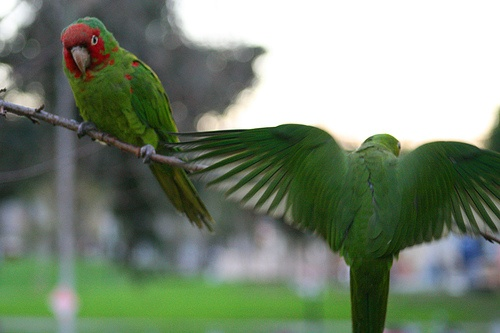
\includegraphics[height=0.1\linewidth]{fig/trimap/2007_000363.jpg} &
%%       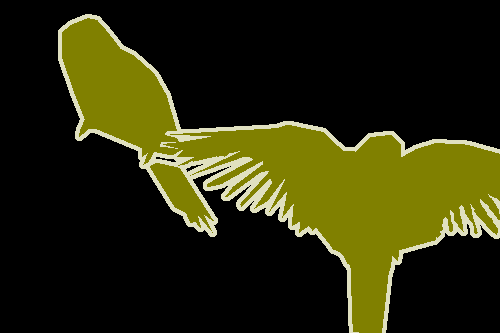
\includegraphics[height=0.1\linewidth]{fig/trimap/2007_000363.png} \\
%%       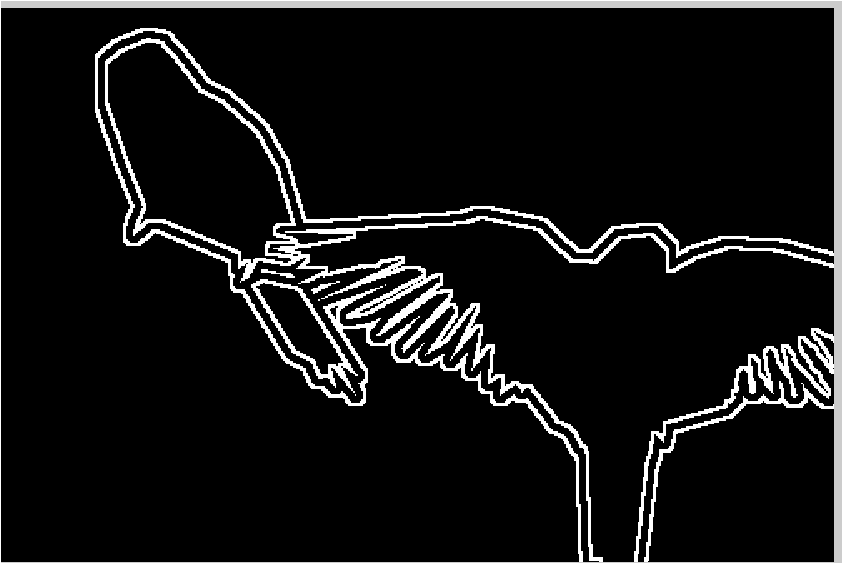
\includegraphics[height=0.1\linewidth]{fig/trimap/TrimapWidth2.pdf} &
%%       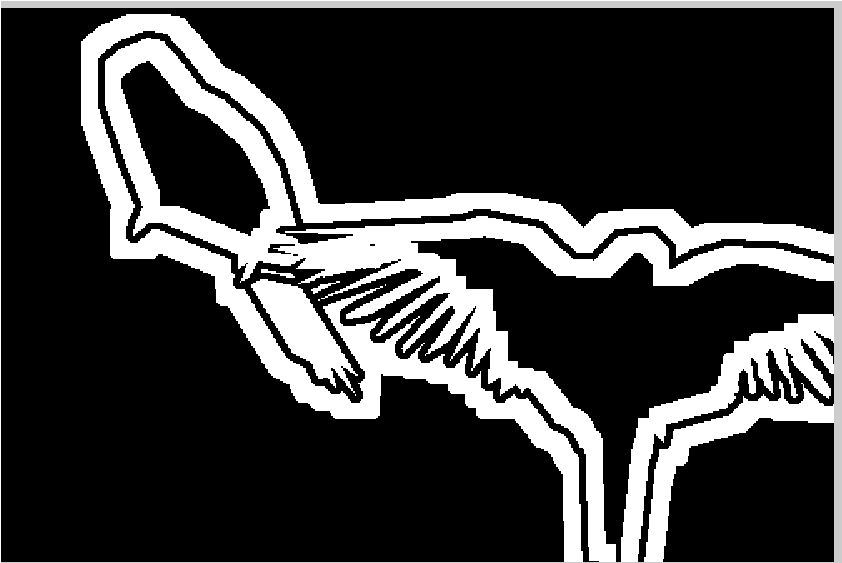
\includegraphics[height=0.1\linewidth]{fig/trimap/TrimapWidth10.pdf} \\
%%     \end{tabular} } &
%%     \includegraphics[height=0.25\linewidth]{fig/SegPixelAccWithinTrimap.pdf} &
%%     \includegraphics[height=0.25\linewidth]{fig/SegPixelIOUWithinTrimap.pdf} \\
%%     (a) & (b) & (c) \\
%%    \end{tabular}
%% }
%%   \caption{(a) Some trimap examples (top-left: image. top-right: ground-truth. bottom-left: trimap of 2 pixels. bottom-right: trimap of 10 pixels). Quality of segmentation result within a band around the object boundaries for the proposed methods. (b) Pixelwise accuracy. (c) Pixel mean IOU. 
%%     }  
%%   \label{fig:IOUBoundary}
%% \end{figure}

%Training time for 10 iterations: 139 sec (7x7) vs. 77 (4x4 hole=8) vs 67 (3x3 hole=12 ave) vs. 62 (3x3 hole=12). But we use batch size = 20 for 7x7 and 4x4, and batch size = 30 for 3x3. 69 sec for 4x4 (hole = 4)


%{\bf{Weighted loss: }} In PASCAL VOC 2012 dataset, most of the pixels are labeled as background in the ground truths. Weighting the loss function according to the class frequency has been employed, \eg \cite{farabet2013learning, mostajabi2014feedforward}, to overcome the label imbalance problem. Our experiments on VOC 2012 val set show that using a weighted loss function increases the mean class accuracy (the pixelwise accuracy averaged across classes), but does not improve the mean IOU in our model. 

%% \begin{figure}[t]
%%   \centering
%%   \begin{tabular}{c c}
%%     \includegraphics[height=0.55\linewidth]{fig/comparedWithFCN.pdf} &
%%     \includegraphics[height=0.55\linewidth]{fig/comparedWithRoomOut.pdf} \\
%%     (a) FCN-8s vs. DeepLab-CRF & (b) TTI-Zoomout-16 vs. DeepLab-CRF \\
%%   \end{tabular}
%%   \caption{Comparisons with state-of-the-art models on the val set. First row: images. Second row: ground truths. Third row: other recent models (Left: FCN-8s, Right: TTI-Zoomout-16). Fourth row: our DeepLab-CRF. Best viewed in color.}
%%   \label{fig:val_comparison}
%% \end{figure}

\textbf{Test set evaluation:} We have evaluated our DeepLab-CRF-LargeFOV model
on the PASCAL VOC 2012 official \textit{test} set. It achieves $70.3\%$ mean IOU
performance.

%% \begin{table}[t]
%%   \centering
%%   \addtolength{\tabcolsep}{2.5pt}
%%   \begin{tabular}{l | c}
%%     \toprule[0.2em]
%%     {\bf Method}      & {\bf mean IOU (\%)} \\
%%     \toprule[0.2em]
%% %    MSRA-CFM    & 61.8 \\
%% %    FCN-8s      & 62.2 \\
%% %    TTI-Zoomout-16 & 64.4 \\
%% %    \midrule \midrule
%%     DeepLab-CRF                 & 66.4 \\
%% %    DeepLab-HC-CRF             & 67.1 \\
%% %    DeepLab-CRF-7x7             & 70.3 \\
%%     DeepLab-CRF-LargeFOV        & 70.3 \\
%% %    DeepLab-CRF-MultiFOV        & 70.6 \\
%% %    DeepLab-HC-CRF-LargeFOV    & 71.6 \\
%%     \bottomrule[0.1em]
%%   \end{tabular}
%%   \caption{Performance of proposed models on the PASCAL VOC 2012 {\it test} set.}
%%   \label{tb:testIOU}
%% \end{table}


%% \begin{table*}[!tbp] %\scriptsize
%% \setlength{\tabcolsep}{3pt}
%% %\hspace{-1.8cm}
%% \resizebox{\columnwidth}{!}{
%% \begin{tabular}{|l||c*{20}{|c}||c|}
%% \hline 
%% Method         & bkg &  aero & bike & bird & boat & bottle& bus & car  &  cat & chair& cow  &table & dog  & horse & mbike& person& plant&sheep& sofa &train & tv   & mean \\
%% \hline \hline
%% MSRA-CFM       & -    & 75.7 & 26.7 & 69.5 & 48.8 & 65.6 & 81.0 & 69.2 & 73.3 & 30.0 & 68.7 & 51.5 & 69.1 & 68.1  & 71.7 & 67.5 & 50.4 & 66.5 & 44.4 & 58.9 & 53.5 & 61.8 \\
%% FCN-8s         & -    & 76.8 & 34.2 & 68.9 & 49.4 & 60.3 & 75.3 & 74.7 & 77.6 & 21.4 & 62.5 & 46.8 & 71.8 & 63.9  & 76.5 & 73.9 & 45.2 & 72.4 & 37.4 & 70.9 & 55.1 & 62.2 \\
%% TTI-Zoomout-16 & 89.8 & 81.9 & 35.1 & 78.2 & 57.4 & 56.5 & 80.5 & 74.0 & 79.8 & 22.4 & 69.6 & 53.7 & 74.0 & 76.0 & 76.6 & 68.8 & 44.3 & 70.2 & 40.2 & 68.9 & 55.3 & 64.4 \\
%% \hline
%% %\href{http://host.robots.ox.ac.uk:8080/anonymous/NTHWZK.html}
%% DeepLab-CRF    & 92.1 & 78.4 & 33.1 & 78.2 & 55.6 & 65.3 & 81.3 & 75.5 & 78.6 & 25.3 & 69.2 & 52.7 & 75.2 & 69.0  & 79.1 & 77.6 & 54.7 & 78.3 & 45.1 & 73.3 & 56.2 & 66.4 \\ 
%% %\href{http://host.robots.ox.ac.uk:8080/anonymous/UQUOMR.html}
%% DeepLab-HC-CRF & 92.6 & 80.4 & 36.8 & 77.4 & 55.2 & 66.4 & 81.5 & 77.5 & 78.9 & 27.1 & 68.2 & 52.7 & 74.3 & 69.6 & 79.4 & 79.0 & 56.9 & 78.8 & 45.2 & 72.7 & 59.3 &  67.1 \\
%% \href{http://host.robots.ox.ac.uk:8080/anonymous/EKRH3N.html}{DeepLab-CRF-7x7} & 92.8 & 83.9 & 36.6 & 77.5 & 58.4 & {\bf 68.0} & 84.6 & {\bf 79.7} & 83.1 & 29.5 & {\bf 74.6} & 59.3 & 78.9 & 76.0 & 82.1 & 80.6 & {\bf 60.3} & 81.7 & 49.2 & {\bf 78.0} & 60.7 & 70.3 \\
%% %\href{http://host.robots.ox.ac.uk:8080/anonymous/0KD2BO.html}
%% DeepLab-CRF-LargeFOV & 92.6 & 83.5 & 36.6 & {\bf 82.5} & 62.3 & 66.5 & {\bf 85.4} & 78.5 & {\bf 83.7} & 30.4 & 72.9 & {\bf 60.4} & 78.5 & 75.5 & 82.1 & 79.7 &  58.2 & 82.0 & 48.8 & 73.7 & 63.3 & 70.3 \\
%% %\href{http://host.robots.ox.ac.uk:8080/anonymous/UPP4XC.html}
%% DeepLab-HC-CRF-LargeFOV & {\bf 93.1} & {\bf 84.4} & {\bf 54.5} & 81.5 & {\bf 63.6} & 65.9 & 85.1 & 79.1 & 83.4 & {\bf 30.7} & 74.1 & 59.8 & {\bf 79.0} & {\bf 76.1} & {\bf 83.2} & {\bf 80.8} & 59.7 & {\bf 82.2} & {\bf 50.4} & 73.1 & {\bf 63.7} & {\bf 71.6} \\
%% \hline
%%  \end{tabular}
%% }
%%  \caption{Labeling IOU (\%) on the PASCAL VOC 2012 test set, using the trainval set for training.}
%%  \label{tab:voc2012}
%% \end{table*}



% \begin{figure}[ht]
%   \centering
%   \begin{tabular}{c c c | c c}
%     \includegraphics[height=0.12\linewidth]{fig/img/2007_002266.jpg} &
%     \includegraphics[height=0.12\linewidth]{fig/fcn8s/2007_002266.png} &
%     \includegraphics[height=0.12\linewidth]{fig/res_crf/2007_002266.png} &
%     \includegraphics[height=0.12\linewidth]{fig/SegPixelAccWithinTrimap_Berkeley.pdf} &
%     \includegraphics[height=0.12\linewidth]{fig/SegPixelIOUWithinTrimap_Berkeley.pdf} \\
%     (a) & (b) & (c) & (d) & (e)
%   \end{tabular}
%   \caption{(Left) Some comparisons with FCN-8S: (a) image; (b) FCN-8S; (c)
%     ms-crf. (d) Segmentation accuracy (pixelwise accuracy) within trimap. (e)
%     Segmentation accuracy (mean IOU) within trimap. {\color{red} TODO: change
%       legend. HELP: I cannot make them equally spaced....}} 
%   \label{fig:IOUBoundary}
% \end{figure}

%% \begin{figure*}[!htbp]
%%   \centering
%%   %\vspace{-1.cm}
%%   \scalebox{0.55} {
%%   \begin{tabular}{c c c | c c c | c c c}
%%     %\addtolength{\tabcolsep}{-6.5pt}
%%     \includegraphics[width=0.18\linewidth]{fig/voc12_val/img/2007_002094.jpg} &
%%     \includegraphics[width=0.18\linewidth]{fig/voc12_val/deeplab/res_none/2007_002094.png} &
%%     \includegraphics[width=0.18\linewidth]{fig/voc12_val/deeplab/res_crf/2007_002094.png} &
%%     \includegraphics[width=0.18\linewidth]{fig/voc12_val/img/2007_002719.jpg} &
%%     \includegraphics[width=0.18\linewidth]{fig/voc12_val/deeplab/res_none/2007_002719.png} &
%%     \includegraphics[width=0.18\linewidth]{fig/voc12_val/deeplab/res_crf/2007_002719.png} &
%%     \includegraphics[width=0.18\linewidth]{fig/voc12_val/img/2007_003957.jpg} &
%%     \includegraphics[width=0.18\linewidth]{fig/voc12_val/deeplab/res_none/2007_003957.png} &
%%     \includegraphics[width=0.18\linewidth]{fig/voc12_val/deeplab/res_crf/2007_003957.png} \\
%%     \includegraphics[width=0.18\linewidth]{fig/voc12_val/img/2007_003991.jpg} &
%%     \includegraphics[width=0.18\linewidth]{fig/voc12_val/deeplab/res_none/2007_003991.png} &
%%     \includegraphics[width=0.18\linewidth]{fig/voc12_val/deeplab/res_crf/2007_003991.png} &
%%     \includegraphics[width=0.18\linewidth]{fig/voc12_val/img/2008_001439.jpg} &
%%     \includegraphics[width=0.18\linewidth]{fig/voc12_val/deeplab/res_none/2008_001439.png} &
%%     \includegraphics[width=0.18\linewidth]{fig/voc12_val/deeplab/res_crf/2008_001439.png} &
%%     \includegraphics[width=0.18\linewidth]{fig/voc12_val/img/2008_004363.jpg} &
%%     \includegraphics[width=0.18\linewidth]{fig/voc12_val/deeplab/res_none/2008_004363.png} &
%%     \includegraphics[width=0.18\linewidth]{fig/voc12_val/deeplab/res_crf/2008_004363.png} \\
%%     \includegraphics[width=0.18\linewidth]{fig/voc12_val/img/2008_006229.jpg} &
%%     \includegraphics[width=0.18\linewidth]{fig/voc12_val/deeplab/res_none/2008_006229.png} &
%%     \includegraphics[width=0.18\linewidth]{fig/voc12_val/deeplab/res_crf/2008_006229.png} &
%%     \includegraphics[width=0.18\linewidth]{fig/voc12_val/img/2009_000421.jpg} &
%%     \includegraphics[width=0.18\linewidth]{fig/voc12_val/deeplab/res_none/2009_000421.png} &
%%     \includegraphics[width=0.18\linewidth]{fig/voc12_val/deeplab/res_crf/2009_000421.png} &
%%     \includegraphics[width=0.18\linewidth]{fig/voc12_val/img/2009_000412.jpg} &
%%     \includegraphics[width=0.18\linewidth]{fig/voc12_val/deeplab/res_none/2009_000412.png} &
%%     \includegraphics[width=0.18\linewidth]{fig/voc12_val/deeplab/res_crf/2009_000412.png} \\
%%     \includegraphics[width=0.18\linewidth]{fig/voc12_val/img/2010_001024.jpg} &
%%     \includegraphics[width=0.18\linewidth]{fig/voc12_val/deeplab/res_none/2010_001024.png} &
%%     \includegraphics[width=0.18\linewidth]{fig/voc12_val/deeplab/res_crf/2010_001024.png} &
%%     \includegraphics[width=0.18\linewidth]{fig/voc12_val/img/2010_001079.jpg} &
%%     \includegraphics[width=0.18\linewidth]{fig/voc12_val/deeplab/res_none/2010_001079.png} &
%%     \includegraphics[width=0.18\linewidth]{fig/voc12_val/deeplab/res_crf/2010_001079.png} &
%%     \includegraphics[width=0.18\linewidth]{fig/voc12_val/img/2007_002852.jpg} &
%%     \includegraphics[width=0.18\linewidth]{fig/voc12_val/deeplab/res_none/2007_002852.png} &
%%     \includegraphics[width=0.18\linewidth]{fig/voc12_val/deeplab/res_crf/2007_002852.png} \\
%%     \includegraphics[width=0.18\linewidth]{fig/voc12_val/img/2007_005331.jpg} &
%%     \includegraphics[width=0.18\linewidth]{fig/voc12_val/deeplab/res_none/2007_005331.png} &
%%     \includegraphics[width=0.18\linewidth]{fig/voc12_val/deeplab/res_crf/2007_005331.png} &
%%     \includegraphics[width=0.18\linewidth]{fig/voc12_val/img/2008_004654.jpg} &
%%     \includegraphics[width=0.18\linewidth]{fig/voc12_val/deeplab/res_none/2008_004654.png} &
%%     \includegraphics[width=0.18\linewidth]{fig/voc12_val/deeplab/res_crf/2008_004654.png} &
%%     \includegraphics[width=0.18\linewidth]{fig/voc12_val/img/2007_000129.jpg} &
%%     \includegraphics[width=0.18\linewidth]{fig/voc12_val/deeplab/res_none/2007_000129.png} &
%%     \includegraphics[width=0.18\linewidth]{fig/voc12_val/deeplab/res_crf/2007_000129.png} \\
%%     %\includegraphics[width=0.18\linewidth]{fig/voc12_val/img/2007_002619.jpg} &
%%     %\includegraphics[width=0.18\linewidth]{fig/voc12_val/deeplab/res_none/2007_002619.png} &
%%     %\includegraphics[width=0.18\linewidth]{fig/voc12_val/deeplab/res_crf/2007_002619.png} &
%%     \includegraphics[width=0.18\linewidth]{fig/voc12_val/img/2009_004504.jpg} &
%%     \includegraphics[width=0.18\linewidth]{fig/voc12_val/deeplab/res_none/2009_004504.png} &
%%     \includegraphics[width=0.18\linewidth]{fig/voc12_val/deeplab/res_crf/2009_004504.png} &
%%     \includegraphics[width=0.18\linewidth]{fig/voc12_val/img/2010_001069.jpg} &
%%     \includegraphics[width=0.18\linewidth]{fig/voc12_val/deeplab/res_none/2010_001069.png} &
%%     \includegraphics[width=0.18\linewidth]{fig/voc12_val/deeplab/res_crf/2010_001069.png} &
%%     \includegraphics[width=0.18\linewidth]{fig/voc12_val/img/2010_000038.jpg} &
%%     \includegraphics[width=0.18\linewidth]{fig/voc12_val/deeplab/res_none/2010_000038.png} &
%%     \includegraphics[width=0.18\linewidth]{fig/voc12_val/deeplab/res_crf/2010_000038.png} \\
%%     %% \hline
%%     %% \hline
%%     %% \includegraphics[width=0.18\linewidth]{fig/voc12_val/img/2007_000491.jpg} &
%%     %% \includegraphics[width=0.18\linewidth]{fig/voc12_val/deeplab/res_none/2007_000491.png} &
%%     %% \includegraphics[width=0.18\linewidth]{fig/voc12_val/deeplab/res_crf/2007_000491.png} &
%%     %% \includegraphics[width=0.18\linewidth]{fig/voc12_val/img/2007_000529.jpg} &
%%     %% \includegraphics[width=0.18\linewidth]{fig/voc12_val/deeplab/res_none/2007_000529.png} &
%%     %% \includegraphics[width=0.18\linewidth]{fig/voc12_val/deeplab/res_crf/2007_000529.png} &
%%     %% \includegraphics[width=0.14\linewidth]{fig/voc12_val/img/2007_000663.jpg} &
%%     %% \includegraphics[width=0.14\linewidth]{fig/voc12_val/deeplab/res_none/2007_000663.png} &
%%     %% \includegraphics[width=0.14\linewidth]{fig/voc12_val/deeplab/res_crf/2007_000663.png} \\    
%%     %% \includegraphics[width=0.18\linewidth]{fig/voc12_val/img/2007_000559.jpg} &
%%     %% \includegraphics[width=0.18\linewidth]{fig/voc12_val/deeplab/res_none/2007_000559.png} &
%%     %% \includegraphics[width=0.18\linewidth]{fig/voc12_val/deeplab/res_crf/2007_000559.png} &
%%     %% \includegraphics[width=0.18\linewidth]{fig/voc12_val/img/2007_000452.jpg} &
%%     %% \includegraphics[width=0.18\linewidth]{fig/voc12_val/deeplab/res_none/2007_000452.png} &
%%     %% \includegraphics[width=0.18\linewidth]{fig/voc12_val/deeplab/res_crf/2007_000452.png} &
%%     %% \includegraphics[width=0.18\linewidth]{fig/voc12_val/img/2007_002268.jpg} &
%%     %% \includegraphics[width=0.18\linewidth]{fig/voc12_val/deeplab/res_none/2007_002268.png} &
%%     %% \includegraphics[width=0.18\linewidth]{fig/voc12_val/deeplab/res_crf/2007_002268.png} \\
%%     (a) Image &
%%     (b) Before CRF &
%%     (c) After CRF &
%%     (a) Image &
%%     (b) Before CRF &
%%     (c) After CRF &
%%     (a) Image &
%%     (b) Before CRF &
%%     (c) After CRF \\
%%   \end{tabular}
%%   }
%%   %\vspace{-0.3cm}
%%   \caption{Visualization of some VOC 2012 \textit{val} results. For each row, we show
%%     the input image, the segmentation result before CRF, and the refined segmentation
%%     result after Fully Connected CRF (DeepLab-CRF). %% We show our failure modes in the last two rows.
%%   }
%%   \label{fig:ValResults}
%% \end{figure*}

% a block to the fc6 with hole = \{2,4,8,12\}. On the validation set, DeepLab has performance 63.67\% (1.42\% improvement over using one hole = 12, \ie, DeepLab-LargeFOV) and DeepLab-CRF yields 67.83\% (0.19\% improvement over DeepLab-CRF-LargeFOV). Similarly, we observe 0.3\% improvment over DeepLab-CRF-LargeFOV on the test set. The improvement of using multiple holes becomes marginal after employing dense CRF, which also has the effect of modeling long-range connection. 


\begin{figure*}[!htbp]
  \centering
  %\vspace{-1.cm}
  \scalebox{0.55} {
  \begin{tabular}{c}
    \includegraphics[width=1.8\linewidth]{fig/voc12_aspp/results.jpg}\\
  \end{tabular}
  }
  %\vspace{-0.3cm}
  \caption{PASCAL VOC 2012 \textit{val} results. Input image
    and our DeepLab results before/after CRF.}
  \label{fig:ValResults}
\end{figure*}


\subsubsection{Improvements after conference version of this work}
After the conference version of this work \cite{chen2014semantic}, we have
pursued three main improvements of our model, which we discuss below:
(1) different learning policy during training, (2) atrous spatial pyramid
pooling, and (3) employment of deeper networks and multi-scale processing.

\textbf{Learning rate policy:} We have explored different learning rate
policies when training DeepLab-LargeFOV. Similar to \cite{liu2015parsenet},
we also found that employing a ``poly'' learning rate policy (the learning
rate is multiplied by $(1-\frac{iter}{max\_iter})^{power}$) is more effective
than ``step'' learning rate (reduce the learning rate at a fixed step size).
As shown in \tabref{tab:val_poly}, employing ``poly'' (with $power = 0.9$)
and using the same batch size and same training iterations yields 1.17\% better
performance than employing ``step'' policy. Fixing the batch size and increasing
the training iteration to 10K improves the performance to 64.90\% (1.48\% gain);
however, the total training time increases due to more training iterations. We
then reduce the batch size to 10 and found that comparable performance is still
maintained (64.90\% \vs 64.71\%). In the end, we employ batch size = 10 and
20K iterations in order to maintain similar training time as previous ``step''
policy. Surprisingly, this gives us the performance of 65.88\% (3.63\%
improvement over ``step'') on \textit{val}, and 67.7\% on \textit{test},
compared to 65.1\% of the original ``step'' setting for DeepLab-LargeFOV before
CRF. We employ the ``poly'' learning rate policy for all experiments reported in
the rest of the paper.

\begin{table}[!t]
  \centering
  \addtolength{\tabcolsep}{2.5pt}
  \begin{tabular}{c c c c}
    \toprule[0.2 em]
    {\bf Learning policy} & {\bf Batch size} & {\bf Iteration} & {\bf mean IOU} \\
    \toprule[0.2em]
    step & 30 & 6K & 62.25 \\
    \midrule
    poly & 30 & 6K & 63.42 \\
    poly & 30 & 10K & 64.90 \\
    poly & 10 & 10K & 64.71 \\
    poly & 10 & 20K & 65.88 \\
    \bottomrule[0.1em]
  \end{tabular}
  \caption{PASCAL VOC 2012 \textit{val} set results (\%) (before CRF) as
    different learning hyper parameters vary. Employing ``poly'' learning
    policy is more effective than ``step'' when training DeepLab-LargeFOV.}
  \label{tab:val_poly}
\end{table}


\begin{figure}[!t]
  \centering
  \scalebox{0.85}{
  \begin{tabular}{c c}
    \includegraphics[width=0.2\linewidth]{./fig/spm/deeplab_largefov.pdf} &
    \includegraphics[height=4.5cm]{./fig/spm/deeplab_spm.pdf} \\
    {\scriptsize (a) DeepLab-LargeFOV} &
    {\scriptsize (b) DeepLab-ASPP} \\
  \end{tabular}
  }
  \caption{DeepLab-ASPP employs multiple filters with different rates to capture objects and context at multiple
    scales.}
  \label{fig:diff_hole}
\end{figure}

\textbf{Atrous Spatial Pyramid Pooling:} We have experimented with the proposed
Atrous Spatial Pyramid Pooling (ASPP) scheme, described in
\secref{sec:convnet-hole}. As shown in \figref{fig:diff_hole}, ASPP for VGG-16
employs several parallel fc6-fc7-fc8 branches. They all use \by{3}{3} kernels
but different atrous rates $r$ in the `fc6' in order to capture objects of
different size. In \tabref{tab:vgg_mfov}, we report results with several
settings:
(1) Our baseline LargeFOV model, having a single branch with $r=12$,
(2) ASPP-S, with four branches and smaller atrous rates ($r$ = \{2, 4, 8, 12\}), and
(3) ASPP-L, with four branches and larger rates ($r$ = \{6, 12, 18, 24\}).
For each variant we report results before and after CRF.
As shown in the table, ASPP-S yields 1.22\% improvement over the baseline
LargeFOV before CRF. However, after CRF both LargeFOV and ASPP-S perform similarly.
On the other hand, ASPP-L yields consistent improvements over the baseline LargeFOV
both before and after CRF. We evaluate on \textit{test} the proposed ASPP-L + CRF
model, attaining 72.6\%. We visualize the effect of the different schemes in
\figref{fig:aspp}.

\begin{table}[!t]
  \centering
  \addtolength{\tabcolsep}{0pt}
  \begin{tabular} {c | c c }
    \toprule[0.2em]
    {\bf Method} & {\bf before CRF} & {\bf after CRF} \\
    \toprule[0.2em]
    LargeFOV & 65.76 & 69.84 \\
    ASPP-S   & 66.98 & 69.73 \\
    ASPP-L   & 68.96 & 71.57 \\
    \bottomrule[0.1em]
  \end{tabular}
  \caption{Effect of ASPP on PASCAL VOC 2012 \textit{val} set
    performance (mean IOU) for VGG-16 based DeepLab model.
    {\bf LargeFOV}: single branch, $r = 12$.
    {\bf ASPP-S}: four branches, $r$ = \{2, 4, 8, 12\}.
    {\bf ASPP-L}: four branches, $r$ = \{6, 12, 18, 24\}.}
  \label{tab:vgg_mfov}
\end{table}

\begin{figure}
  \centering
  \begin{tabular}{c c c c}
    \includegraphics[width=0.21\linewidth]{fig/spm/img/2010_003947.jpg} &
    \includegraphics[width=0.21\linewidth]{fig/spm/vgg128_noup_pool3_20M_largewin3_newcode5/post_none/2010_003947.png} &
    \includegraphics[width=0.21\linewidth]{fig/spm/vgg128_noup_pool3_40M_largewin_spm_2/post_none/2010_003947.png} &    
    \includegraphics[width=0.21\linewidth]{fig/spm/vgg128_noup_pool3_40M_largewin_spm_3/post_none/2010_003947.png} \\
    \includegraphics[width=0.21\linewidth]{fig/spm/img/2010_003446.jpg} &
    \includegraphics[width=0.21\linewidth]{fig/spm/vgg128_noup_pool3_20M_largewin3_newcode5/post_none/2010_003446.png} &
    \includegraphics[width=0.21\linewidth]{fig/spm/vgg128_noup_pool3_40M_largewin_spm_2/post_none/2010_003446.png} &    
    \includegraphics[width=0.21\linewidth]{fig/spm/vgg128_noup_pool3_40M_largewin_spm_3/post_none/2010_003446.png} \\
    (a) Image &
    (b) LargeFOV &
    (c) ASPP-S &
    (d) ASPP-L \\
  \end{tabular}
  \caption{Qualitative segmentation results with ASPP compared to the baseline
    LargeFOV model. The \textbf{ASPP-L} model, employing multiple {\it large}
    FOVs can successfully capture objects as well as image context at multiple
    scales.}
  \label{fig:aspp}
\end{figure}


\begin{table}[!t]
  \centering
  \addtolength{\tabcolsep}{-1pt}
  \begin{tabular} {c c c c c c | c}
    \toprule[0.2em]
    {\bf MSC} & {\bf COCO} & {\bf Aug} & {\bf LargeFOV} & {\bf ASPP} & {\bf CRF} & {\bf mIOU} \\
    \toprule[0.2em]
    %\multicolumn{7}{l}{\it VGG-16 net}  \\
    %DeepLab-LargeFOV \cite{chen2014semantic} & 62.25 \\
    %DeepLab-LargeFOV-Max \cite{chen2015attention}& 67.79 \\
    %DeepLab-LargeFOV-COCO \cite{papandreou2015weakly} & 67.58 \\
    %DeepLab \cite{chen2015attention} & \check & \check & & \check 70.06 \\
    %\midrule
    %\multicolumn{7}{l}{\it ResNet-101} & \\
    & & & & & & 68.72 \\
    \checkmark & & & & & & 71.27 \\
    \checkmark & \checkmark & & & & & 73.28 \\
%    DeepLab-COCO & 73.50 \\
    \checkmark & \checkmark & \checkmark & & & & 74.87 \\
    %DeepLab-CRF-Max-COCO+ & & & & & & 75.95 \\
    \checkmark & \checkmark & \checkmark & \checkmark & & & 75.54 \\
    \checkmark & \checkmark & \checkmark & & \checkmark & & 76.35 \\
    \checkmark & \checkmark & \checkmark & & \checkmark & \checkmark & 77.69 \\
    \bottomrule[0.1em]
  \end{tabular}
  \caption{Employing ResNet-101 for DeepLab on PASCAL VOC 2012 {\it val} set.
    {\bf MSC}: Employing mutli-scale inputs with max fusion.
    {\bf COCO}: Models pretrained on MS-COCO.
    {\bf Aug}: Data augmentation by randomly rescaling inputs.}
  \label{tab:resnet_val}
\end{table}

\textbf{Deeper Networks and Multiscale Processing:} We have experimented
building DeepLab around the recently proposed residual net ResNet-101
\cite{he2015deep} instead of VGG-16. Similar to what we did for VGG-16 net,
we re-purpose ResNet-101 by atrous convolution, as described in
\secref{sec:convnet-hole}. On top of that, we adopt several other features,
following recent work of \cite{farabet2013learning, papandreou2015weakly,
  zheng2015conditional, liu2015semantic, lin2015efficient, chen2015attention,
  kokkinos2016pushing}: (1) Multi-scale inputs: We separately feed to the
DCNN images at scale = \{0.5, 0.75, 1\}, fusing their score maps by taking
the maximum response across scales for each position separately
\cite{chen2015attention}. (2) Models pretrained on MS-COCO
\cite{lin2014microsoft}. (3) Data augmentation by randomly scaling the input
images (from 0.5 to 1.5) during training. In \tabref{tab:resnet_val}, we
evaluate how each of these factors, along with LargeFOV and atrous spatial
pyramid pooling (ASPP), affects \textsl{val} set performance.
Adopting ResNet-101 instead of VGG-16 significantly improves DeepLab performance
(\eg, our simplest ResNet-101 based model attains 68.72\%, compared to 65.76\%
of our DeepLab-LargeFOV VGG-16 based variant, both before CRF). Multiscale
fusion \cite{chen2015attention} brings extra 2.55\% improvement, while
pretraining the model on MS-COCO gives another 2.01\% gain. Data augmentation
during training is effective (about 1.6\% improvement). Employing LargeFOV
(adding an atrous convolutional layer on top of ResNet, with \by{3}{3} kernel
and rate = 12) is beneficial (about 0.6\% improvement). Further 0.8\%
improvement is achieved by atrous spatial pyramid pooling (ASPP).
Post-processing our best model by dense CRF yields performance of 77.69\%.

%We report the performance on the validation set in \tabref{tab:resnet_val}. As shown in the table, adopting ResNet-101 for DeepLab significantly outperform the performance when employing VGG-16 net. 
%Following the recent work of , we employ as input an image pyramid (specifically, images with scale = \{0.5, 0.75, 1\}). Similar to \cite{chen2015attention}, we also use extra supervision and max-pooling to merge the results from all the scales. The method proposed by \cite{chen2015attention} exploits the multi-scale features (by scaling the input images) more efficiently while only one-step end-to-end training of the DeepLab part is required. Please refer to \cite{chen2015attention} for details.
%We denote the model, adopting the multi-scale inputs and max-pooling to merge the results \cite{chen2015attention}, as DeepLab-Max. In that case, DeepLab-Max (ResNet-101) outperform DeepLab-LargeFOV-Max (VGG-16) by 3.48\%. Pretraining the model on the MS-COCO dataset \cite{lin2014microsoft} gives extra 2\% improvement (denoted as DeepLab-Max-COCO). Similar to \cite{lin2015efficient}, augmenting the dataset by randomly scaling the input images (from 0.5 to 1.5) during training brings about 1.6\% more improvement (denoted as DeepLab-Max-COCO+). After incorporating dense CRF as post processing, our model, DeepLab-CRF-Max-COCO+, achieves the performance of 75.95\% on the validation set. Note that we observe adopting ResNet-52 \cite{he2015deep} has worse performance than ResNet-101, while ResNet-152 has similar performance to ResNet-101 but with longer processing time for each image. We, thus, adopt ResNet-101 for all the experiments. 

\textbf{Qualitative results:} We provide qualitative visual comparisons of DeepLab's
results (our best model variant) before and after CRF in \figref{fig:ValResults}.
The visualization results obtained by DeepLab before CRF already yields excellent
segmentation results, while employing the CRF further improves the performance by
removing false positives and refining object boundaries. 


%We conduct the majority of our evaluations
%on the \textit{val} set, training our model on the \textit{trainaug} set.
%We note that the work of
%\cite{krahenbuhl2011efficient} improved the $27.6\%$ result of TextonBoost
%\cite{shotton2009textonboost} to $29.1\%$, which makes the improvement we report
%here (from $59.8\%$ to $63.7\%$) all the more impressive.
%We provide qualitative visual comparisons of DeepLab's
%results before and after CRF in \figref{fig:ValResults}. Employing the CRF
%leads to significant qualitative improvements, allowing the model to accurately
%capture intricate object boundaries.

\textbf{Test set results:} We have submitted the result of our final best model
to the official server, obtaining \textit{test} set performance of 79.7\%, as
shown in \tabref{tab:res_testset}. The model substantially outperforms previous
DeepLab variants (\eg, DeepLab-LargeFOV with VGG-16 net) and is currently the
top performing method on the PASCAL VOC 2012 segmentation leaderboard. 

%, and is comparable with concurrent work \cite{wu2016high} which further employs on-line hard example mining. 
%% We have observed a marginal further 0.3\% improvement by adopting an ensemble
%% approach \cite{szegedy2014going, he2015deep, noh2015learning, liu2015semantic}.
%% Averaging the results of two ASPP models (one trained on \textit{trainval} and
%% another on \textit{trainvalaug}), we achieve 79.6\% on the test set. Integrating
%% into our model other advanced methods (\eg, joint training of DCNN and CRF
%% \cite{zheng2015conditional,arnab2015higher}, four step training \cite{liu2015semantic},
%% and non-linear pairwise term \cite{lin2015efficient}) could lead to further improvements.

\begin{table}[!th]
  \centering
  \addtolength{\tabcolsep}{2.5pt}
  \begin{tabular}{l | c}
    \toprule[0.2 em]
    {\bf Method} & {\bf mIOU} \\
    \toprule[0.2 em]
    %DeepLab-LargeFOV-COCO (VGG-16 net) \cite{papandreou2015weakly} & 68.9\\
    %\midrule
    DeepLab-CRF-LargeFOV-COCO \cite{papandreou2015weakly} & 72.7\\
    MERL\_DEEP\_GCRF \cite{Vemulapalli2016Gaussian} & 73.2 \\
    CRF-RNN \cite{zheng2015conditional} & 74.7 \\
    POSTECH\_DeconvNet\_CRF\_VOC \cite{noh2015learning} & 74.8 \\
    BoxSup \cite{dai2015boxsup} & 75.2 \\
    Context + CRF-RNN \cite{yu2015multi} & 75.3 \\
    $QO_4^{mres}$ \cite{chandra2016fast} & 75.5 \\
    DeepLab-CRF-Attention \cite{chen2015attention} & 75.7 \\
    CentraleSuperBoundaries++ \cite{kokkinos2016pushing} & 76.0 \\
    DeepLab-CRF-Attention-DT  \cite{chen2015semantic} & 76.3 \\
    H-ReNet + DenseCRF \cite{yan2016combining} & 76.8 \\
    LRR\_4x\_COCO \cite{ghiasi2016laplacian} & 76.8 \\
    DPN \cite{liu2015semantic} & 77.5 \\
    Adelaide\_Context \cite{lin2015efficient} & 77.8 \\
    Oxford\_TVG\_HO\_CRF \cite{arnab2015higher} & 77.9 \\
    Context CRF + Guidance CRF \cite{Shen2016Fast} & 78.1 \\
    Adelaide\_VeryDeep\_FCN\_VOC \cite{wu2016bridging} & 79.1 \\
    \midrule
    \href{http://host.robots.ox.ac.uk:8080/anonymous/FLHY8R.html}{DeepLab-CRF (ResNet-101)} & 79.7 \\
%    \href{http://host.robots.ox.ac.uk:8080/anonymous/SV4ESR.html}{Ensemble DeepLab-CRF (ResNet-101)} & 79.6 \\
    \bottomrule[0.1 em]
  \end{tabular}
  \caption{Performance on PASCAL VOC 2012 {\it test} set. We have added some
    results from recent arXiv papers on top of the official leadearboard results.}
  \label{tab:res_testset}
\end{table}

\textbf{VGG-16 \vs ResNet-101:} We have observed that DeepLab based on ResNet-101 \cite{he2015deep}
delivers better segmentation results along object boundaries than employing VGG-16 \cite{simonyan2014very}, as
visualized in \figref{fig:res_vs_vgg_results}. We think the identity mapping \cite{he2016identity} of ResNet-101
has similar effect as hyper-column features \cite{hariharan2014hypercolumns}, which exploits the features from
the intermediate layers to better localize boundaries. We further quantize this effect in \figref{fig:IOUBoundary} within the
``trimap'' \cite{kohli2009robust, krahenbuhl2011efficient} (a narrow band along object boundaries). As shown in
the figure, employing ResNet-101 before CRF has almost the same accuracy along object boundaries as employing
VGG-16 in conjunction with a CRF. Post-processing the ResNet-101 result with a CRF further improves the segmentation
result.

\begin{figure}[!t]
  \centering
  %\vspace{-1.cm}
  \scalebox{0.85} {
  \begin{tabular}{c @{\hskip 5pt} c @{\hskip 5pt} c @{\hskip 5pt} c @{\hskip 5pt} c}
    %%\addtolength{\tabcolsep}{10pt}
    %% \includegraphics[width=0.18\linewidth]{fig/res_vs_vgg/resnet101_noup_pool3_14/img/2007_000129.jpg} &
    %% \includegraphics[width=0.18\linewidth]{fig/res_vs_vgg/vgg128_noup_pool3_20M_largewin3_newcode5/res_none/2007_000129.png} &
    %% \includegraphics[width=0.18\linewidth]{fig/res_vs_vgg/vgg128_noup_pool3_20M_largewin3_newcode5/res_crf/2007_000129.png} &
    %% \includegraphics[width=0.18\linewidth]{fig/res_vs_vgg/resnet101_noup_pool3_14/res_none/2007_000129.png} &
    %% \includegraphics[width=0.18\linewidth]{fig/res_vs_vgg/resnet101_noup_pool3_14/res_crf/2007_000129.png} \\

    %% \includegraphics[width=0.18\linewidth]{fig/res_vs_vgg/resnet101_noup_pool3_14/img/2008_006874.jpg} &
    %% \includegraphics[width=0.18\linewidth]{fig/res_vs_vgg/vgg128_noup_pool3_20M_largewin3_newcode5/res_none/2008_006874.png} &
    %% \includegraphics[width=0.18\linewidth]{fig/res_vs_vgg/vgg128_noup_pool3_20M_largewin3_newcode5/res_crf/2008_006874.png} &
    %% \includegraphics[width=0.18\linewidth]{fig/res_vs_vgg/resnet101_noup_pool3_14/res_none/2008_006874.png} &
    %% \includegraphics[width=0.18\linewidth]{fig/res_vs_vgg/resnet101_noup_pool3_14/res_crf/2008_006874.png} \\

    \includegraphics[width=0.21\linewidth]{fig/res_vs_vgg/resnet101_noup_pool3_14/img/2007_001311.jpg} &
    \includegraphics[width=0.21\linewidth]{fig/res_vs_vgg/vgg128_noup_pool3_20M_largewin3_newcode5/res_none/2007_001311.png} &
    \includegraphics[width=0.21\linewidth]{fig/res_vs_vgg/vgg128_noup_pool3_20M_largewin3_newcode5/res_crf/2007_001311.png} &
    \includegraphics[width=0.21\linewidth]{fig/res_vs_vgg/resnet101_noup_pool3_14/res_none/2007_001311.png} &
    \includegraphics[width=0.21\linewidth]{fig/res_vs_vgg/resnet101_noup_pool3_14/res_crf/2007_001311.png} \\

    \includegraphics[width=0.21\linewidth]{fig/res_vs_vgg/resnet101_noup_pool3_14/img/2011_000455.jpg} &
    \includegraphics[width=0.21\linewidth]{fig/res_vs_vgg/vgg128_noup_pool3_20M_largewin3_newcode5/res_none/2011_000455.png} &
    \includegraphics[width=0.21\linewidth]{fig/res_vs_vgg/vgg128_noup_pool3_20M_largewin3_newcode5/res_crf/2011_000455.png} &
    \includegraphics[width=0.21\linewidth]{fig/res_vs_vgg/resnet101_noup_pool3_14/res_none/2011_000455.png} &
    \includegraphics[width=0.21\linewidth]{fig/res_vs_vgg/resnet101_noup_pool3_14/res_crf/2011_000455.png} \\

    {\scriptsize Image} &
    {\scriptsize VGG-16 Bef.} &
    {\scriptsize VGG-16 Aft.} &
    {\scriptsize ResNet Bef.} &
    {\scriptsize ResNet Aft.} \\
  \end{tabular}
  }
  %\vspace{-0.3cm}
  \caption{DeepLab results based on VGG-16 net or ResNet-101 before and after CRF.
    The CRF is critical for accurate prediction along object boundaries with VGG-16, whereas
    ResNet-101 has acceptable performance even before CRF.}
  \label{fig:res_vs_vgg_results}
\end{figure}

\begin{figure}[!t]
\centering
\resizebox{\columnwidth}{!}{
  \begin{tabular} {c c}
%    \hspace{-0.5cm}\raisebox{2cm}
    \raisebox{1cm} {
    \begin{tabular}{c c}
      \includegraphics[height=0.1\linewidth]{fig/trimap/2007_000363.jpg} &
      \includegraphics[height=0.1\linewidth]{fig/trimap/2007_000363.png} \\
      \includegraphics[height=0.1\linewidth]{fig/trimap/TrimapWidth2.pdf} &
      \includegraphics[height=0.1\linewidth]{fig/trimap/TrimapWidth10.pdf} \\
    \end{tabular} } &
    \includegraphics[height=0.25\linewidth]{fig/res_vs_vgg/SegPixelIOUWithinTrimap_ResVsVGG} \\
    (a) & (b) \\
   \end{tabular}
}
  \caption{(a) Trimap examples (top-left: image. top-right: ground-truth. bottom-left: trimap of 2 pixels.
    bottom-right: trimap of 10 pixels). (b) Pixel mean IOU as a function of the band width around the
    object boundaries when employing VGG-16 or ResNet-101 before and after CRF.}
  \label{fig:IOUBoundary}
\end{figure}


\subsection{PASCAL-Context}
\label{exp:pascal_context}

\begin{figure*}[!t]
  \centering
  %\vspace{-1.cm}
  \scalebox{0.9} {
  \begin{tabular}{c}
    \includegraphics[width=1\linewidth]{fig/pascal_context/results.jpg} \\
  \end{tabular}
  }
  \caption{PASCAL-Context results. Input image, ground-truth,
    and our DeepLab results before/after CRF.}
  \label{fig:pascal_context_val_results}
\end{figure*}

\begin{table}[!t]
  \centering
  \addtolength{\tabcolsep}{-3pt}
  \begin{tabular} {l c c c c c c | c}
    \toprule[0.2 em]
    {\bf Method} & {\bf MSC} & {\bf COCO} & {\bf Aug} & {\bf LargeFOV} & {\bf ASPP} & {\bf CRF} & {\bf mIOU} \\
    \toprule[0.2 em]
    \multicolumn{7}{l}{\it VGG-16} & \\
    DeepLab \cite{chen2014semantic}& & & &\checkmark & & & 37.6 \\
    DeepLab \cite{chen2014semantic}& & & &\checkmark & & \checkmark  &  39.6 \\
    \midrule
    \multicolumn{7}{l}{\it ResNet-101} & \\
    DeepLab & & & & & & &  39.6 \\
    DeepLab &\checkmark & & \checkmark & & & &  41.4 \\
    DeepLab &\checkmark &\checkmark & \checkmark & & & &  42.9 \\
    DeepLab &\checkmark &\checkmark & \checkmark & \checkmark & & & 43.5 \\
    DeepLab &\checkmark &\checkmark & \checkmark & & \checkmark & & 44.7 \\
    DeepLab &\checkmark &\checkmark & \checkmark & & \checkmark & \checkmark & 45.7 \\
%    DeepLab-CRF-Max (ResNet-101) & 43.1 \\
%    DeepLab-CRF-Max-COCO (ResNet-101) & 44.5 \\
    \midrule \midrule
    $O_2P$ \cite{carreira2012semantic}& & & & & &  & 18.1 \\
    CFM \cite{dai2014convolutional}& & & & & &  & 34.4 \\
    FCN-8s \cite{long2014fully}& & & & & &  & 37.8 \\
    CRF-RNN \cite{zheng2015conditional}& & & & & &  & 39.3 \\
    ParseNet \cite{liu2015parsenet}& & & & & &  & 40.4 \\
    BoxSup \cite{dai2015boxsup}& & & & & &  & 40.5 \\
    HO\_CRF \cite{arnab2015higher}& & & & & &  & 41.3 \\
    Context \cite{lin2015efficient}& & & & & &  & 43.3 \\
    VeryDeep \cite{wu2016bridging}& & & & & &  & 44.5 \\
    \bottomrule[0.1 em]
  \end{tabular}
  \caption{Comparison with other state-of-art methods on PASCAL-Context dataset.}
  \label{tab:pascal_context}
\end{table}

\textbf{Dataset:} The PASCAL-Context dataset \cite{mottaghi2014role} provides
detailed semantic labels for the whole scene, including both object (\eg, person)
and stuff (\eg, sky). Following \cite{mottaghi2014role}, the proposed models are
evaluated on the most frequent 59 classes along with one background category.
The training set and validation set contain 4998 and 5105 images.

\textbf{Evaluation:} We report the evaluation results in \tabref{tab:pascal_context}.
Our VGG-16 based LargeFOV variant yields 37.6\% before and 39.6\% after CRF.
Repurposing the ResNet-101 \cite{he2015deep} for DeepLab improves 2\% over the
VGG-16 LargeFOV. Similar to \cite{chen2015attention}, employing multi-scale inputs
and max-pooling to merge the results improves the performance to 41.4\%.
Pretraining the model on MS-COCO brings extra 1.5\% improvement.
Employing atrous spatial pyramid pooling is more effective than LargeFOV.
After further employing dense CRF as post processing, our final model
yields 45.7\%, outperforming the current state-of-art method
\cite{lin2015efficient} by 2.4\% without using their non-linear pairwise term. Our final
model is slightly better than the concurrent work \cite{wu2016bridging} by 1.2\%, which also employs
atrous convolution to repurpose the residual net of \cite{he2015deep} for semantic segmentation.

\textbf{Qualitative results:} We visualize the segmentation results of our best
model with and without CRF as post processing in
\figref{fig:pascal_context_val_results}. DeepLab before CRF can already predict
most of the object/stuff with high accuracy. Employing CRF, our model is able to
further remove isolated false positives and improve the prediction along
object/stuff boundaries.

\subsection{PASCAL-Person-Part}
\label{exp:pascal_person_part}

\begin{figure*}[!th]
  \centering
  %\vspace{-1.cm}
  \scalebox{0.9} {
  \begin{tabular}{c}
    \includegraphics[width=1.\linewidth]{fig/voc10_part/results.jpg} \\
  \end{tabular}
  }
  \caption{PASCAL-Person-Part results. Input image, ground-truth,
    and our DeepLab results before/after CRF.}
  \label{fig:voc10_part_val_results}
\end{figure*}

\begin{table}[!t]
  \centering
  \addtolength{\tabcolsep}{-3pt}
  \begin{tabular} {l  c c c c c c | c}
    \toprule[0.2 em]
    {\bf Method} & {\bf MSC} & {\bf COCO} & {\bf Aug} & {\bf LFOV} & {\bf ASPP} & {\bf CRF} & {\bf mIOU} \\
    \toprule[0.2 em]
    \multicolumn{7}{l}{\it ResNet-101} & \\
    DeepLab      & & & & & & & 58.90 \\
    DeepLab      & \checkmark & & \checkmark & & & & 63.10 \\
    DeepLab      & \checkmark & \checkmark & \checkmark & & & & 64.40 \\
    DeepLab      & \checkmark & \checkmark & \checkmark & & & \checkmark & 64.94 \\
    \midrule
    DeepLab      & \checkmark & \checkmark & \checkmark & \checkmark & & & 62.18 \\
    DeepLab      & \checkmark & \checkmark & \checkmark & & \checkmark & & 62.76 \\
    \midrule \midrule
%    DeepLab-LargeFOV  \cite{chen2015attention} & & & & & & & 51.91 \\
    Attention \cite{chen2015attention} & & & & & & & 56.39 \\
    HAZN \cite{xia2015zoom} & & & & & &  & 57.54 \\
    LG-LSTM \cite{liang2015semantic} & & & & & &  & 57.97 \\
    Graph LSTM \cite{liang2016semantic} & & & & & &  & 60.16 \\
    \bottomrule[0.1 em]
  \end{tabular}
  \caption{Comparison with other state-of-art methods on PASCAL-Person-Part dataset.}
  \label{tab:pascal_person_part}
\end{table}

\textbf{Dataset:} We further perform experiments on semantic part segmentation \cite{wang2014semantic, wang2015joint},
using the extra PASCAL VOC 2010 annotations by \cite{chen_cvpr14}. We focus on the
{\it person} part for the dataset, which contains more training data and large
variation in object scale and human pose. Specifically, the dataset contains
detailed part annotations for every person, \eg eyes, nose. We merge the
annotations to be Head, Torso, Upper/Lower Arms and Upper/Lower Legs, resulting
in six person part classes and one background class. We only use those images
containing persons for training (1716 images) and validation (1817 images).

\textbf{Evaluation:} The human part segmentation results on PASCAL-Person-Part is
reported in \tabref{tab:pascal_person_part}. \cite{chen2015attention} has already
conducted experiments on this dataset with re-purposed VGG-16 net for DeepLab,
attaining 56.39\% (with multi-scale inputs). Therefore, in this part, we mainly
focus on the effect of repurposing ResNet-101 for DeepLab. With ResNet-101,
DeepLab alone yields 58.9\%, significantly outperforming DeepLab-LargeFOV
(VGG-16 net) and DeepLab-Attention (VGG-16 net) by about 7\% and 2.5\%,
respectively. Incorporating multi-scale inputs and fusion by max-pooling
further improves performance to 63.1\%. Additionally pretraining the model on
MS-COCO yields another 1.3\% improvement. However, we do not observe any
improvement when adopting either LargeFOV or ASPP on this dataset. Employing
the dense CRF to post process our final output substantially outperforms the
concurrent work \cite{liang2016semantic} by 4.78\%.

\textbf{Qualitative results:} We visualize the results in \figref{fig:voc10_part_val_results}.

\subsection{Cityscapes}
\label{exp:cityscapes}

\begin{figure*}[!t]
  \centering
  %\vspace{-1.cm}
  \scalebox{1} {
  \begin{tabular}{c}
    \includegraphics[width=0.9\linewidth]{fig/cityscapes/results.jpg} \\
    %% \includegraphics[width=0.23\linewidth]{fig/cityscapes/frankfurt/resnet101_noup_pool3_7/img/frankfurt_000001_007857_img.png} &
    %% \includegraphics[width=0.23\linewidth]{fig/cityscapes/frankfurt/resnet101_noup_pool3_7/gt/frankfurt_000001_007857_labelImg.png} &
    %% \includegraphics[width=0.23\linewidth]{fig/cityscapes/frankfurt/resnet101_noup_pool3_7/res_none/frankfurt_000001_007857_gtFine_labelTrainIds.png} &
    %% \includegraphics[width=0.23\linewidth]{fig/cityscapes/frankfurt/resnet101_noup_pool3_7/res_crf/frankfurt_000001_007857_gtFine_labelTrainIds.png} \\

    %% \includegraphics[width=0.23\linewidth]{fig/cityscapes/frankfurt/resnet101_noup_pool3_7/img/frankfurt_000001_025512_img.png} &
    %% \includegraphics[width=0.23\linewidth]{fig/cityscapes/frankfurt/resnet101_noup_pool3_7/gt/frankfurt_000001_025512_labelImg.png} &
    %% \includegraphics[width=0.23\linewidth]{fig/cityscapes/frankfurt/resnet101_noup_pool3_7/res_none/frankfurt_000001_025512_gtFine_labelTrainIds.png} &
    %% \includegraphics[width=0.23\linewidth]{fig/cityscapes/frankfurt/resnet101_noup_pool3_7/res_crf/frankfurt_000001_025512_gtFine_labelTrainIds.png} \\

    %% \includegraphics[width=0.23\linewidth]{fig/cityscapes/frankfurt/resnet101_noup_pool3_7/img/frankfurt_000000_013067_img.png} &
    %% \includegraphics[width=0.23\linewidth]{fig/cityscapes/frankfurt/resnet101_noup_pool3_7/gt/frankfurt_000000_013067_labelImg.png} &
    %% \includegraphics[width=0.23\linewidth]{fig/cityscapes/frankfurt/resnet101_noup_pool3_7/res_none/frankfurt_000000_013067_gtFine_labelTrainIds.png} &
    %% \includegraphics[width=0.23\linewidth]{fig/cityscapes/frankfurt/resnet101_noup_pool3_7/res_crf/frankfurt_000000_013067_gtFine_labelTrainIds.png} \\

    %% %% \includegraphics[width=0.23\linewidth]{fig/cityscapes/frankfurt/resnet101_noup_pool3_7/img/frankfurt_000001_066832_img.png} &
    %% %% \includegraphics[width=0.23\linewidth]{fig/cityscapes/frankfurt/resnet101_noup_pool3_7/gt/frankfurt_000001_066832_labelImg.png} &
    %% %% \includegraphics[width=0.23\linewidth]{fig/cityscapes/frankfurt/resnet101_noup_pool3_7/res_none/frankfurt_000001_066832_gtFine_labelTrainIds.png} &
    %% %% \includegraphics[width=0.23\linewidth]{fig/cityscapes/frankfurt/resnet101_noup_pool3_7/res_crf/frankfurt_000001_066832_gtFine_labelTrainIds.png} \\

    %% %% \includegraphics[width=0.23\linewidth]{fig/cityscapes/frankfurt/resnet101_noup_pool3_7/img/frankfurt_000001_015768_img.png} &
    %% %% \includegraphics[width=0.23\linewidth]{fig/cityscapes/frankfurt/resnet101_noup_pool3_7/gt/frankfurt_000001_015768_labelImg.png} &
    %% %% \includegraphics[width=0.23\linewidth]{fig/cityscapes/frankfurt/resnet101_noup_pool3_7/res_none/frankfurt_000001_015768_gtFine_labelTrainIds.png} &
    %% %% \includegraphics[width=0.23\linewidth]{fig/cityscapes/frankfurt/resnet101_noup_pool3_7/res_crf/frankfurt_000001_015768_gtFine_labelTrainIds.png} \\

    %% %% \includegraphics[width=0.23\linewidth]{fig/cityscapes/frankfurt/resnet101_noup_pool3_7/img/frankfurt_000001_046504_img.png} &
    %% %% \includegraphics[width=0.23\linewidth]{fig/cityscapes/frankfurt/resnet101_noup_pool3_7/gt/frankfurt_000001_046504_labelImg.png} &
    %% %% \includegraphics[width=0.23\linewidth]{fig/cityscapes/frankfurt/resnet101_noup_pool3_7/res_none/frankfurt_000001_046504_gtFine_labelTrainIds.png} &
    %% %% \includegraphics[width=0.23\linewidth]{fig/cityscapes/frankfurt/resnet101_noup_pool3_7/res_crf/frankfurt_000001_046504_gtFine_labelTrainIds.png} \\

    %% {\scriptsize (a) Image} &
    %% {\scriptsize (b) G.T.} &
    %% {\scriptsize (c) Before CRF} &
    %% {\scriptsize (d) After CRF} \\
  \end{tabular}
  }
  \caption{Cityscapes results. Input image, ground-truth,
    and our DeepLab results before/after CRF.}
  \label{fig:cityscapes_val_results}
\end{figure*}


\begin{table}[!t]
  \centering
  \addtolength{\tabcolsep}{2.5pt}
  \begin{tabular}{l | c}
    \toprule[0.2 em]
    {\bf Method} & {\bf mIOU} \\
    \toprule[0.2 em]
    \multicolumn{2}{l}{\it pre-release version of dataset} \\
    Adelaide\_Context \cite{lin2015efficient} & 66.4 \\
    FCN-8s \cite{long2014fully} & 65.3 \\
    \midrule
    DeepLab-CRF-LargeFOV-StrongWeak \cite{papandreou2015weakly} & 64.8 \\
    DeepLab-CRF-LargeFOV \cite{chen2014semantic} & 63.1 \\
    \midrule
    CRF-RNN \cite{zheng2015conditional} & 62.5 \\
    DPN \cite{liu2015semantic} & 59.1 \\
    Segnet basic \cite{badrinarayanan2015segnet} & 57.0 \\
    Segnet extended \cite{badrinarayanan2015segnet} & 56.1 \\
    \midrule \midrule
    \multicolumn{2}{l}{\it official version} \\
    Adelaide\_Context \cite{lin2015efficient} & 71.6 \\
    Dilation10 \cite{yu2015multi} & 67.1 \\
    DPN \cite{liu2015semantic} & 66.8  \\
    Pixel-level Encoding \cite{uhrig2016pixel} & 64.3 \\
    \midrule
    DeepLab-CRF (ResNet-101) & 70.4 \\
    \bottomrule[0.1 em]
  \end{tabular}
  \caption{Test set results on the Cityscapes dataset, comparing our DeepLab system with other state-of-art methods.}
  \label{tab:cityscapes_test}
\end{table}

\begin{table}[!t]
  \centering
  \addtolength{\tabcolsep}{2pt}
  \begin{tabular}{c c c c c | c}
    \toprule[0.2 em]
    {\bf Full} & {\bf Aug} & {\bf LargeFOV} & {\bf ASPP} & {\bf CRF} & {\bf mIOU} \\
    \toprule[0.2 em]
    \multicolumn{5}{l}{\it VGG-16} & \\
    & & \checkmark & & & 62.97 \\
    & & \checkmark & & \checkmark & 64.18 \\
    \checkmark & & \checkmark & & & 64.89 \\
    \checkmark & & \checkmark & & \checkmark & 65.94 \\
    \midrule
    \multicolumn{5}{l}{\it ResNet-101} & \\
    \checkmark & & & & & 66.6 \\
    \checkmark & & \checkmark & & & 69.2 \\
    \checkmark & &  & \checkmark & & 70.4 \\
    \checkmark & \checkmark & & \checkmark & & 71.0 \\
    \checkmark & \checkmark & & \checkmark & \checkmark & 71.4 \\
    \midrule
%    DeepLab-LargeFOV (full-res) & 64.89 \\
%    DeepLab-CRF-LargeFOV (full-res) & 65.94 \\
%    DeepLab-LargeFOV (full-res + pretrained) & 65.19 \\
%    DeepLab-CRF-LargeFOV (full-res + pretrained) & 66.09 \\
    \bottomrule[0.1 em]
  \end{tabular}
  \caption{Val set results on Cityscapes dataset. {\bf Full}: model trained with full resolution images.}
  \label{tab:cityscapes_val_resnet}
\end{table}

\textbf{Dataset:} Cityscapes \cite{Cordts2016Cityscapes} is a recently released
large-scale dataset, which contains high quality pixel-level annotations of 5000
images collected in street scenes from 50 different cities. Following the
evaluation protocol \cite{Cordts2016Cityscapes}, 19 semantic labels (belonging
to 7 super categories: ground, construction, object, nature, sky, human, and
vehicle) are used for evaluation (the void label is not considered for
evaluation). The training, validation, and test sets contain 2975, 500, and
1525 images respectively.

\textbf{Test set results of pre-release:} We have participated in benchmarking
the Cityscapes dataset pre-release. As shown in the top of \tabref{tab:cityscapes_test},
our model attained third place, with performance of 63.1\% and 64.8\% (with training on
additional coarsely annotated images). 

\textbf{Val set results:} After the initial release, we further explored the
validation set in \tabref{tab:cityscapes_val_resnet}. The images of Cityscapes
have resolution \by{2048}{1024}, making it a challenging problem to train deeper
networks with limited GPU memory. During benchmarking the pre-release of the dataset,
we downsampled the images by 2. However, we have found that it is beneficial to
process the images in their original resolution. With the same training protocol,
using images of original resolution significantly brings 1.9\% and 1.8\% improvements
before and after CRF, respectively. In order to perform inference on this dataset with
high resolution images, we split each image into overlapped regions, similar to
\cite{Cordts2016Cityscapes}. We have also replaced the VGG-16 net with ResNet-101.
We do not exploit multi-scale inputs due to the limited GPU memories at hand.
Instead, we only explore (1) deeper networks (\ie, ResNet-101), (2) data augmentation,
(3) LargeFOV or ASPP, and (4) CRF as post processing on this dataset. We first find
that employing ResNet-101 alone is better than using VGG-16 net. Employing LargeFOV
brings 2.6\% improvement and using ASPP further improves results by 1.2\%.
Adopting data augmentation and CRF as post processing brings another 0.6\% and 0.4\%,
respectively.

\textbf{Current test result:} We have uploaded our best model to the evaluation server,
obtaining performance of 70.4\%. Note that our model is only trained on the train set.

\textbf{Qualitative results:} We visualize the results in \figref{fig:cityscapes_val_results}.

\subsection{Failure Modes}
We further qualitatively analyze some failure modes of our best model variant on PASCAL VOC 2012 {\it val} set. As shown in \figref{fig:failure_modes}, our proposed model fails to capture the delicate boundaries of objects, such as bicycle and chair. The details could not even be recovered by the CRF post processing since the unary term is not confident enough. We hypothesize the encoder-decoder structure of 
\cite{badrinarayanan2015segnet, ronneberger2015u} may alleviate the problem by exploiting the high resolution feature maps in the decoder path. How to efficiently incorporate the method is left as a future work.


\begin{figure}[!t]
\centering
\resizebox{\columnwidth}{!}{
  \begin{tabular} {c c c c}
    \includegraphics[width=0.24\linewidth]{fig/failure_mode/voc12/resnet101_noup_pool3_coco_22/img/2007_000572.jpg} &
    \includegraphics[width=0.24\linewidth]{fig/failure_mode/voc12/resnet101_noup_pool3_coco_22/gt/2007_000572.png} &
    \includegraphics[width=0.24\linewidth]{fig/failure_mode/voc12/resnet101_noup_pool3_coco_22/before_crf/2007_000572.png} &
    \includegraphics[width=0.24\linewidth]{fig/failure_mode/voc12/resnet101_noup_pool3_coco_22/after_crf/2007_000572.png} \\
    \includegraphics[width=0.24\linewidth]{fig/failure_mode/voc12/resnet101_noup_pool3_coco_22/img/2009_002487.jpg} &
    \includegraphics[width=0.24\linewidth]{fig/failure_mode/voc12/resnet101_noup_pool3_coco_22/gt/2009_002487.png} &
    \includegraphics[width=0.24\linewidth]{fig/failure_mode/voc12/resnet101_noup_pool3_coco_22/before_crf/2009_002487.png} &
    \includegraphics[width=0.24\linewidth]{fig/failure_mode/voc12/resnet101_noup_pool3_coco_22/after_crf/2009_002487.png} \\
                    {\scriptsize (a) Image} &
                    {\scriptsize (b) G.T.} &
                    {\scriptsize (c) Before CRF} &
                    {\scriptsize (d) After CRF} \\
  \end{tabular}

}
  \caption{Failure modes. Input image, ground-truth, and our DeepLab results before/after CRF.}  
  \label{fig:failure_modes}
\end{figure}

\section{Conclusion}
我们提出的 ``DeepLab'' 系统通过将 ``空洞卷积'' 与上采样滤波器一起应用于密集特征提取,将图像分类训练的系统重新用于语义分割任务。我们进一步将其扩展到空洞空间金字塔池化,它在多个尺度上捕获对象以及图像上下文。为了沿对象边界生成语义准确的预测和详细的分割图,我们还结合了深度卷积神经网络和全连接的条件随机场。我们的实验结果表明,该方法在几个具有挑战性的数据集中显著提升了现有技术水平,包括 PASCAL VOC 2012、PASCAL-Context、PASCAL-Person-Part、Cityscapes 数据集。

\section*{Acknowledgments}
本工作由 ARO 62250-CS, FP7-RECONFIG, FP7-MOBOT, and H2020-ISUPPORT EU 项目支持。我们诚挚地感谢 NVIDIA 企业为我们的研究提供 GPU 设备支持。


%% % if have a single appendix:
%% %\appendix[Proof of the Zonklar Equations]
%% % or
%% %\appendix  % for no appendix heading
%% % do not use \section anymore after \appendix, only \section*
%% % is possibly needed

%% % use appendices with more than one appendix
%% % then use \section to start each appendix
%% % you must declare a \section before using any
%% % \subsection or using \label (\appendices by itself
%% % starts a section numbered zero.)
%% %


%% \appendices
%% \section{Proof of the First Zonklar Equation}
%% Appendix one text goes here.

%% % you can choose not to have a title for an appendix
%% % if you want by leaving the argument blank
%% \section{}
%% Appendix two text goes here.


%%%%%%%%% uncomment to add acknowledgements
%% % use section* for acknowledgment
%% \ifCLASSOPTIONcompsoc
%%   % The Computer Society usually uses the plural form
%%   \section*{Acknowledgments}
%% \else
%%   % regular IEEE prefers the singular form
%%   \section*{Acknowledgment}
%% \fi


%% The authors would like to thank...





% Can use something like this to put references on a page
% by themselves when using endfloat and the captionsoff option.
\ifCLASSOPTIONcaptionsoff
  \newpage
\fi



% trigger a \newpage just before the given reference
% number - used to balance the columns on the last page
% adjust value as needed - may need to be readjusted if
% the document is modified later
%\IEEEtriggeratref{8}
% The "triggered" command can be changed if desired:
%\IEEEtriggercmd{\enlargethispage{-5in}}

% references section

% can use a bibliography generated by BibTeX as a .bbl file
% BibTeX documentation can be easily obtained at:
% http://mirror.ctan.org/biblio/bibtex/contrib/doc/
% The IEEEtran BibTeX style support page is at:
% http://www.michaelshell.org/tex/ieeetran/bibtex/
%\bibliographystyle{IEEEtran}
% argument is your BibTeX string definitions and bibliography database(s)
%\bibliography{IEEEabrv,../bib/paper}
%
% <OR> manually copy in the resultant .bbl file
% set second argument of \begin to the number of references
% (used to reserve space for the reference number labels box)


{
\bibliographystyle{IEEEtran}
\bibliography{./egbib}
}
%\begin{thebibliography}{1}
%\bibitem{IEEEhowto:kopka}
%H.~Kopka and P.~W. Daly, \emph{A Guide to {\LaTeX}}, 3rd~ed.\hskip 1em plus
%  0.5em minus 0.4em\relax Harlow, England: Addison-Wesley, 1999.
%\end{thebibliography}


% biography section
% 
% If you have an EPS/PDF photo (graphicx package needed) extra braces are
% needed around the contents of the optional argument to biography to prevent
% the LaTeX parser from getting confused when it sees the complicated
% \includegraphics command within an optional argument. (You could create
% your own custom macro containing the \includegraphics command to make things
% simpler here.)
%\begin{IEEEbiography}[{\includegraphics[width=1in,height=1.25in,clip,keepaspectratio]{mshell}}]{Michael Shell}
% or if you just want to reserve a space for a photo:

\begin{IEEEbiography}[{\includegraphics[width=1in,height=1.25in,keepaspectratio]{./fig/bio/jay.jpg}}]{Liang-Chieh Chen}
received his B.Sc. from National Chiao Tung University, Taiwan, his M.S. from the University of Michigan- Ann Arbor, and his
Ph.D. from the University of California- Los Angeles. He is currently working at Google. His research interests
include semantic image segmentation, probabilistic graphical models, and machine learning.
\end{IEEEbiography}

\begin{IEEEbiography}[{\includegraphics[width=1in,height=1.25in,keepaspectratio]{./fig/bio/gpapan.png}}]{George Papandreou}
(S'03--M'09--SM'14) holds a Diploma (2003) and a Ph.D. (2009) in Electrical
Engineering and Computer Science, both from the National Technical University
of Athens (NTUA), Greece. He is currently a Research Scientist at Google,
following appointments as Research Assistant Professor at the Toyota
Technological Institute at Chicago (2013-2014) and Postdoctoral Research Scholar
at the University of California, Los Angeles (2009-2013).

His research interests are in computer vision and machine learning, with a
current emphasis on deep learning. He regularly serves as a reviewer and
program committee member to the main journals and conferences in computer
vision, image processing, and machine learning. He has been a co-organizer of
the NIPS 2012, 2013, and 2014 Workshops on Perturbations, Optimization, and
Statistics and co-editor of a book on the same topic (MIT Press, 2016).
\end{IEEEbiography}

\begin{IEEEbiography}[{\includegraphics[width=1in,height=1.25in,keepaspectratio]{./fig/bio/iasonas.png}}]{Iasonas Kokkinos}
(S'02--M'06) obtained the Diploma of Engineering in 2001 and the Ph.D. Degree in 2006 from the School of Electrical and Computer Engineering of the National Technical University of Athens in Greece, and the Habilitation Degree in 2013 from Université Paris-Est. In 2006 he joined the University of California at Los Angeles as a postdoctoral scholar, and in 2008 joined as faculty the Department of Applied Mathematics of Ecole Centrale Paris (CentraleSupelec), working an associate professor in the Center for Visual Computing of CentraleSupelec and affiliate researcher at INRIA-Saclay. In 2016 he joined University College London and Facebook Artificial Intelligence Research. His currently research activity is on deep learning for computer vision, focusing in particular on structured prediction for deep learning, shape modeling, and multi-task learning architectures. He has been awarded a young researcher grant by the French National Research Agency, has served as associate editor for the Image and Vision Computing and Computer Vision and Image Understanding Journals, serves regularly as a reviewer and area chair for all major computer vision conferences and journals.
\end{IEEEbiography}

\begin{IEEEbiography}[{\includegraphics[width=1in,height=1.25in,keepaspectratio]{./fig/bio/kmurphy.png}}]{Kevin Murphy}
was born in Ireland, grew
up  in  England,  went  to  graduate  school  in  the
USA (MEng from U. Penn, PhD from UC Berkeley,
Postdoc at MIT), and then became a professor at
the Computer Science and Statistics Departments at
the University of British Columbia in
Vancouver, Canada in 2004. After getting tenure,
Kevin  went  to  Google  in  Mountain  View,  California
for his sabbatical. In 2011, he converted
to a full-time research scientist at Google. Kevin
has published over 50 papers in refereed conferences
and journals related to machine learning and graphical models.
He  has  recently  published  an  1100-page  textbook  called
``Machine Learning: a Probabilistic Perspective''
(MIT Press, 2012).
\end{IEEEbiography}

\begin{IEEEbiography}[{\includegraphics[width=1in,height=1.25in,keepaspectratio]{./fig/bio/alan.jpg}}]{Alan L. Yuille}
(F'09) received the BA degree in math-
ematics from the University of Cambridge in
1976. His PhD on theoretical physics, super-
vised by Prof. S.W. Hawking, was approved
in 1981. He was a research scientist in the
Artificial Intelligence Laboratory at MIT and
the Division of Applied Sciences at Harvard
University  from  1982  to  1988.  He  served
as  an  assistant  and  associate  professor  at
Harvard  until  1996.  He  was  a  senior  research scientist at the Smith-Kettlewell Eye
Research Institute from 1996 to 2002. He joined the University of
California, Los Angeles, as a full professor with a joint appointment
in  statistics  and  psychology  in  2002, and computer  science  in  2007. 
He was appointed a Bloomberg Distinguished Professor at Johns Hopkins University in January 2016.
He holds a joint appointment between the Departments of Cognitive science and Computer Science. 
His  research  interests  include
computational models of vision, mathematical models of cognition,
and artificial intelligence and neural network
\end{IEEEbiography}

%% \begin{IEEEbiography}{Michael Shell}
%% Biography text here.
%% \end{IEEEbiography}

%% % if you will not have a photo at all:
%% \begin{IEEEbiographynophoto}{John Doe}
%% Biography text here.
%% \end{IEEEbiographynophoto}

%% % insert where needed to balance the two columns on the last page with
%% % biographies
%% %\newpage

%% \begin{IEEEbiographynophoto}{Jane Doe}
%% Biography text here.
%% \end{IEEEbiographynophoto}

%% % You can push biographies down or up by placing
%% % a \vfill before or after them. The appropriate
%% % use of \vfill depends on what kind of text is
%% % on the last page and whether or not the columns
%% % are being equalized.

%% %\vfill

%% % Can be used to pull up biographies so that the bottom of the last one
%% % is flush with the other column.
%% %\enlargethispage{-5in}


% that's all folks
\end{document}


